\chapter{CUTLASS 教程：Blackwell GEMM-使用线程块cluster}

\begin{center}\small 作者：赵尚春（知乎 @tongsanpang，专栏「CUDA-365」）\quad 原文：\url{https://zhuanlan.zhihu.com/p/2007758781354897660}\end{center}

% 转换章内部放宽断行：原文含大量无自然断点的长标识符，避免 \hbox 溢出（只在本章生效）
\begingroup\setlength{\emergencystretch}{2em}

本文翻译自：\url{https://research.colfax-intl.com/cutlass-tutorial-gemm-with-thread-block-clusters-on-nvidia-blackwell-gpus/}

欢迎来到我们探索 NVIDIA Blackwell 架构上 GEMM 系列的第二部分。在第一部分中，我们介绍了 NVIDIA Blackwell GPU 上的一些关键新特性，包括 Tensor Memory，并讲解了如何编写一个简单的 CUTLASS GEMM 核心，该核心使用新的 UMMA 指令（\texttt{tcgen05.\allowbreak{}mma}）来调用 Blackwell 张量核心。在本文中，我们将解释如何为 Blackwell GEMM 利用线程块cluster和 2-SM UMMA。更具体地说，我们将按顺序涵盖以下几个方面：

\begin{enumerate}
\item 将 Tensor Memory Accelerator (TMA) 与线程块cluster和多播结合使用，在参与的 CTA 之间分担全局内存传输；
\item 使用 Blackwell 2-SM UMMA 与 CTA 对来提高 MMA 的算术强度；
\item 在 GEMM 主循环中同时使用 TMA 多播和 2-SM UMMA，并正确地同步这些操作。
\end{enumerate}

与上一篇博客一样，我们将首先深入讨论相关概念，然后通过 Cu\allowbreak{}Te Blackwell 示例（\url{https://github.com/NVIDIA/cutlass/tree/main/examples/cute/tutorial/blackwell}，具体是示例 3 和 4）了解如何在 CUTLASS 中实现它们。这两个示例与我们介绍概念的顺序一致——第三个示例演示了使用 TMA 多播和 Blackwell 1-SM UMMA 的 GEMM，而第四个示例将其扩展到使用 CTA 对和新的同步原语（包括不同的多播 TMA 原子）的 2-SM UMMA。

\section{线程块cluster}

线程块cluster是一种结构，允许开发人员将物理上靠近（例如，在片上）的 SM 分组。具体来说，cluster中的线程块保证被共同调度到位于同一 GPU 处理cluster（GPC）上的 SM 上。

\begin{figure}[H]\centering
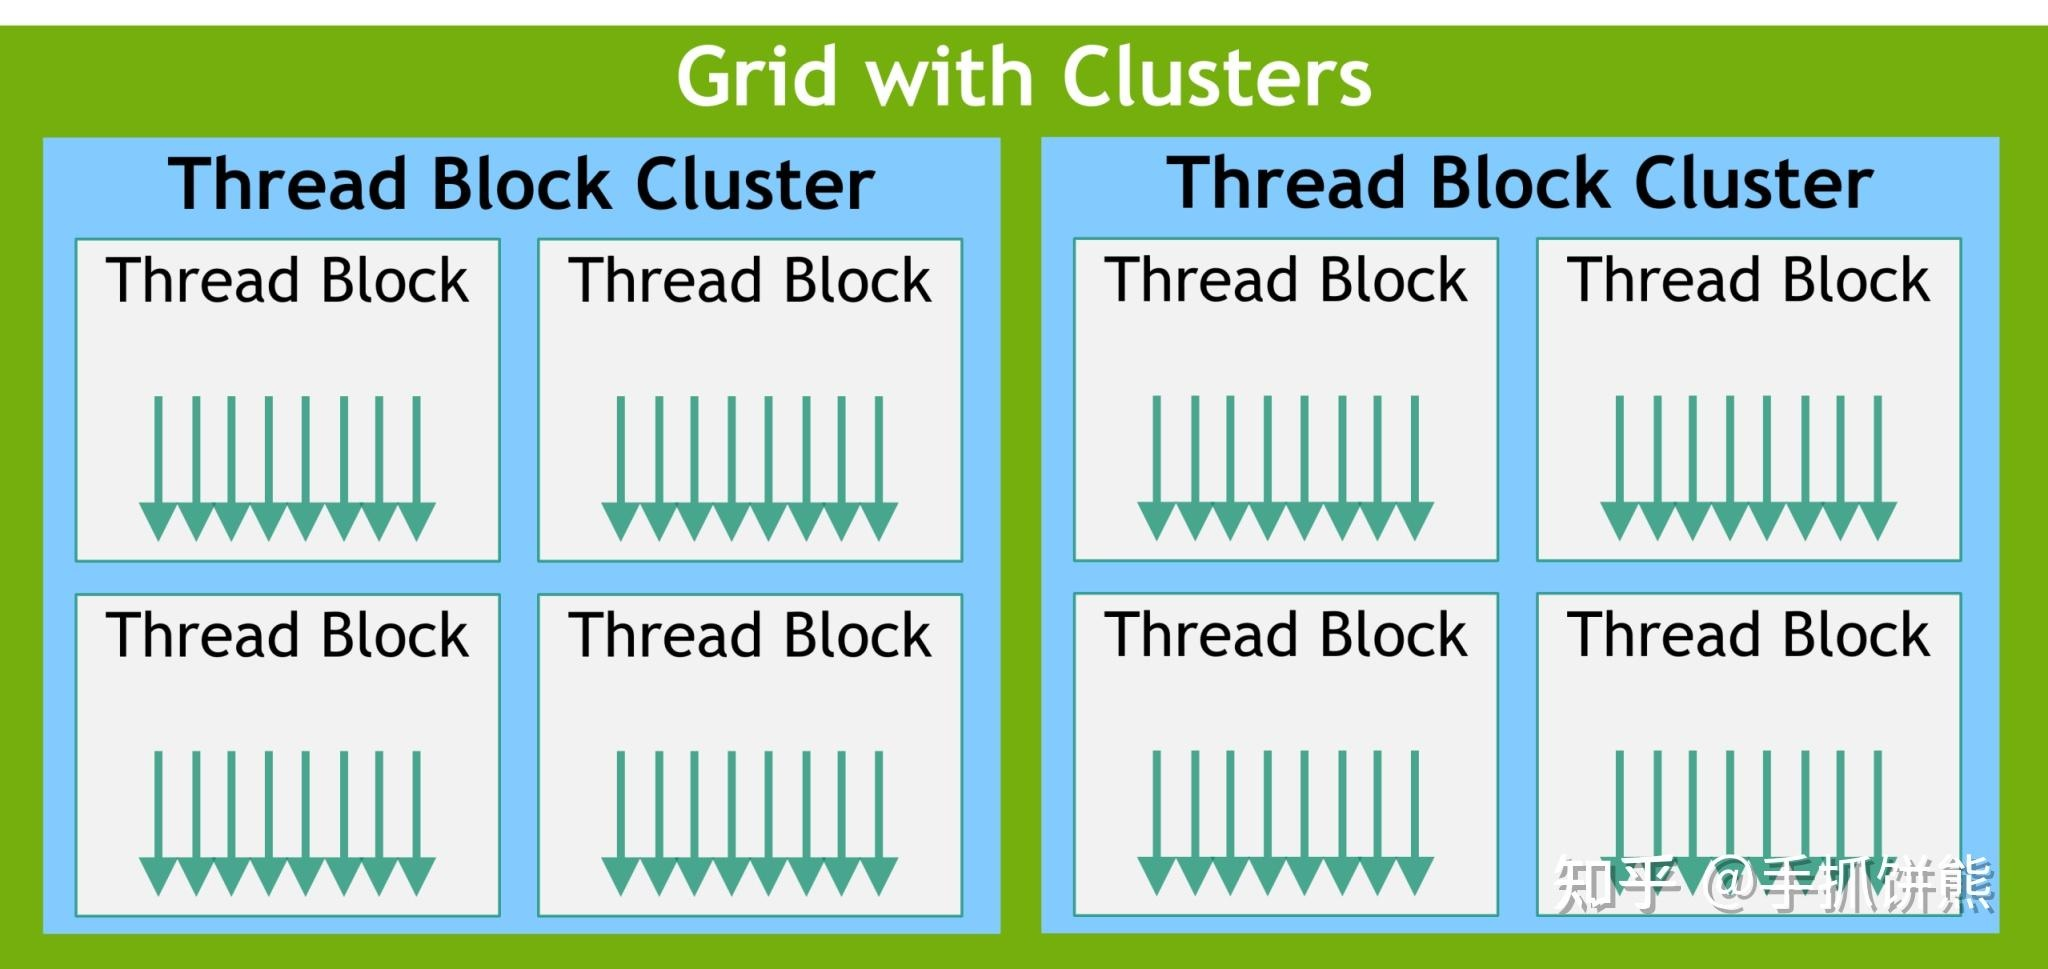
\includegraphics[width=\textwidth]{figures/zhaoshangchun-02-cluster-gemm/fig-01.jpg}
\caption{图 1. 组织成cluster的线程块网格图，来自 CUDA C++ 编程指南。}
\end{figure}

此特性首次在 NVIDIA Hopper 架构中引入，为开发人员提供了新层次的层次结构，以促进相邻线程块之间更高级的合作。值得注意的是，cluster中的线程块可以访问彼此的共享内存，这种能力称为\textbf{分布式共享内存}。这也使得cluster中的线程块能够协作加载数据（例如，通过 TMA 多播），并使用共同可见的 mbarrier 相互同步。我们将在稍后的博客中看到这些特性的实际应用。

\subsection{使用线程块cluster}

线程块cluster是一个启动时参数，就像网格大小或块大小一样。cluster大小以 \texttt{dim3} 元组 \texttt{<\allowbreak{}c\allowbreak{}l\allowbreak{}u\allowbreak{}s\allowbreak{}t\allowbreak{}e\allowbreak{}r\allowbreak{}.\allowbreak{}x\allowbreak{},\allowbreak{} \allowbreak{}c\allowbreak{}l\allowbreak{}u\allowbreak{}s\allowbreak{}t\allowbreak{}e\allowbreak{}r\allowbreak{}.\allowbreak{}y\allowbreak{},\allowbreak{} \allowbreak{}c\allowbreak{}l\allowbreak{}u\allowbreak{}s\allowbreak{}t\allowbreak{}e\allowbreak{}r\allowbreak{}.\allowbreak{}z\allowbreak{}>} 定义。支持的最大可移植cluster大小为 8，尽管某些 GPU（如 Hopper H100 和 Blackwell B200）允许通过选择加入选项将cluster大小扩展到 16。我们将最小形状 \texttt{<1,\allowbreak{}1,\allowbreak{}1>} 的cluster称为\textbf{平凡}cluster。最后，cluster形状必须能够整除网格大小。

在 CUTLASS 中，我们使用一个特殊的启动工具 \texttt{launch\_\allowbreak{}kernel\_\allowbreak{}on\_\allowbreak{}cluster} 来启动cluster。

\begin{figure}[H]\centering
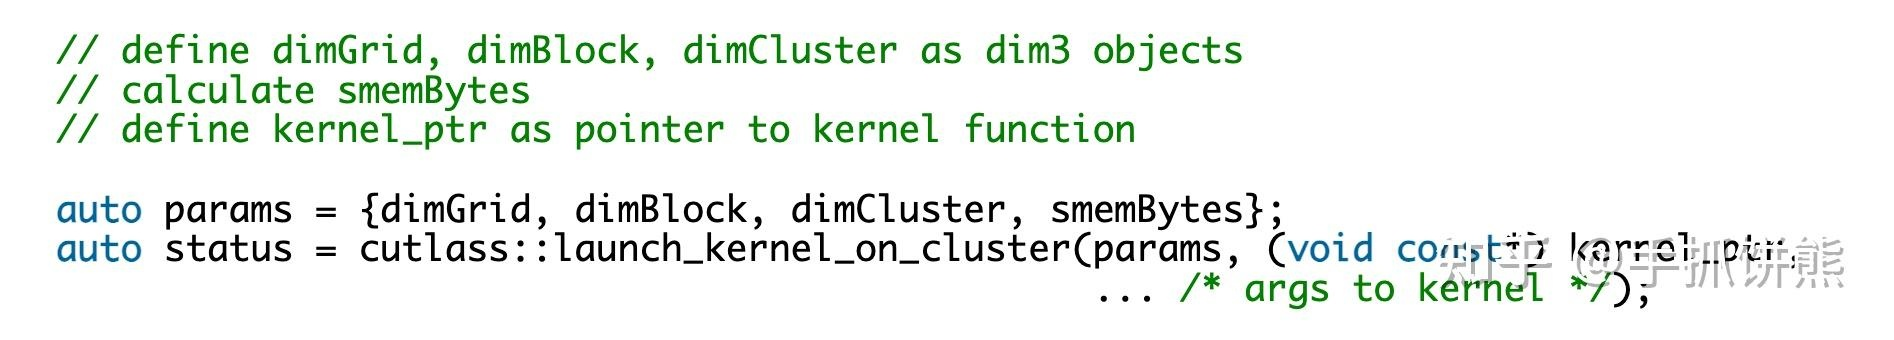
\includegraphics[width=\textwidth]{figures/zhaoshangchun-02-cluster-gemm/fig-02.jpg}
\end{figure}

在 GEMM 核心中，很自然地将cluster形状的三个维度映射到问题的三个维度（M、N、K）（cluster形状的 K 维度等于 1，除非使用 Split-K 核心设计）。这意味着每个cluster中的 CTA 被分配了一个连续的输出分片块，这有利于缓存性能，并且正如我们稍后将看到的，也有利于多播。

\subsection{TMA 多播}

TMA 多播加载是一种旨在通过一次将相同的张量分片加载到同一cluster中的多个 CTA 来加速数据传输的特性。此特性与线程块cluster和 TMA 一起在 Hopper 中引入，我们已在之前的博客文章中介绍过。

简要回顾一下，TMA 多播将 TMA 加载的数据放置在同一个cluster中多个 CTA 的 SMEM 中。使用此特性，cluster中的一组 CTA 可以协作并同时将一个数据分片加载到它们各自的共享内存中，从而在多个 CTA 需要加载相同数据的情况下减少全局内存流量。每个 CTA 加载数据的一部分，这些数据会被多播到其他参与 CTA 的 SMEM 中。例如，如果参与的 CTA 数量为 4，则每个 CTA 加载数据的四分之一，从而将使用 TMA 加载的总数据量减少 4 倍。从技术上讲，这种协作式部分加载是一种编程范式，并非 TMA 多播特性固有的，但在本文中，我们将它们视为同义词。

\section{CuTe 示例：使用 TMA 多播的 GEMM}

现在让我们看一下 \textbf{Cu\allowbreak{}Te Blackwell 示例 3 （}\url{https://github.com/NVIDIA/cutlass/blob/main/examples/cute/tutorial/blackwell/03_mma_tma_multicast_sm100.cu}），看看多播是如何在 GEMM 上下文中使用的。多播自然地适用于 GEMM 的分块方案，因为操作数 A 和 B 中的每个分片都用于计算多个输出分片。为简单起见，让我们首先考虑一个形状为 \texttt{<2,\allowbreak{}2,\allowbreak{}1>} 的cluster（注意，实际示例使用的是形状 \texttt{<4,\allowbreak{}4,\allowbreak{}1>}）。每个 CTA 处理一个大小为 \texttt{(b\allowbreak{}M,\allowbreak{} b\allowbreak{}N)} 的输出分片，因此每个cluster处理一个 2×2 的 4 个输出分片块，总大小为 \texttt{(2*b\allowbreak{}M,\allowbreak{} 2*b\allowbreak{}N)}。

在每个主循环迭代中，每个 CTA 必须从 A 加载一个 \texttt{(b\allowbreak{}M,\allowbreak{} b\allowbreak{}K)} 分片，从 B 加载一个 \texttt{(b\allowbreak{}N,\allowbreak{} b\allowbreak{}K)} 分片，分片的 M 和 N 偏移量由该 CTA 在网格中的行和列决定，K 偏移量由迭代决定。如果我们使用简单的 TMA，每个输出分片将加载 2 个分片，导致cluster加载 8 个分片。虽然像 CTA 光栅化这样的优化可以确保这些加载大部分来自 L2，但很难达到 100\% 的命中率，而且即使 L2 命中，在 MMA 操作的时间尺度上也有显著的延迟。TMA 多播允许我们只加载最低要求的 4 个分片，并将它们放置在需要它们的 CTA 的 SMEM 中。更准确地说，每个 CTA 需要的 A 操作数分片与同一行中的所有其他 CTA 相同，需要的 B 操作数分片与同一列中的所有其他 CTA 相同。因此，每个 CTA 参与两个 TMA 多播操作——一个用于操作数 A，与同一行的所有其他 CTA 一起；一个用于操作数 B，与同一列的所有其他 CTA 一起。

\begin{figure}[H]\centering
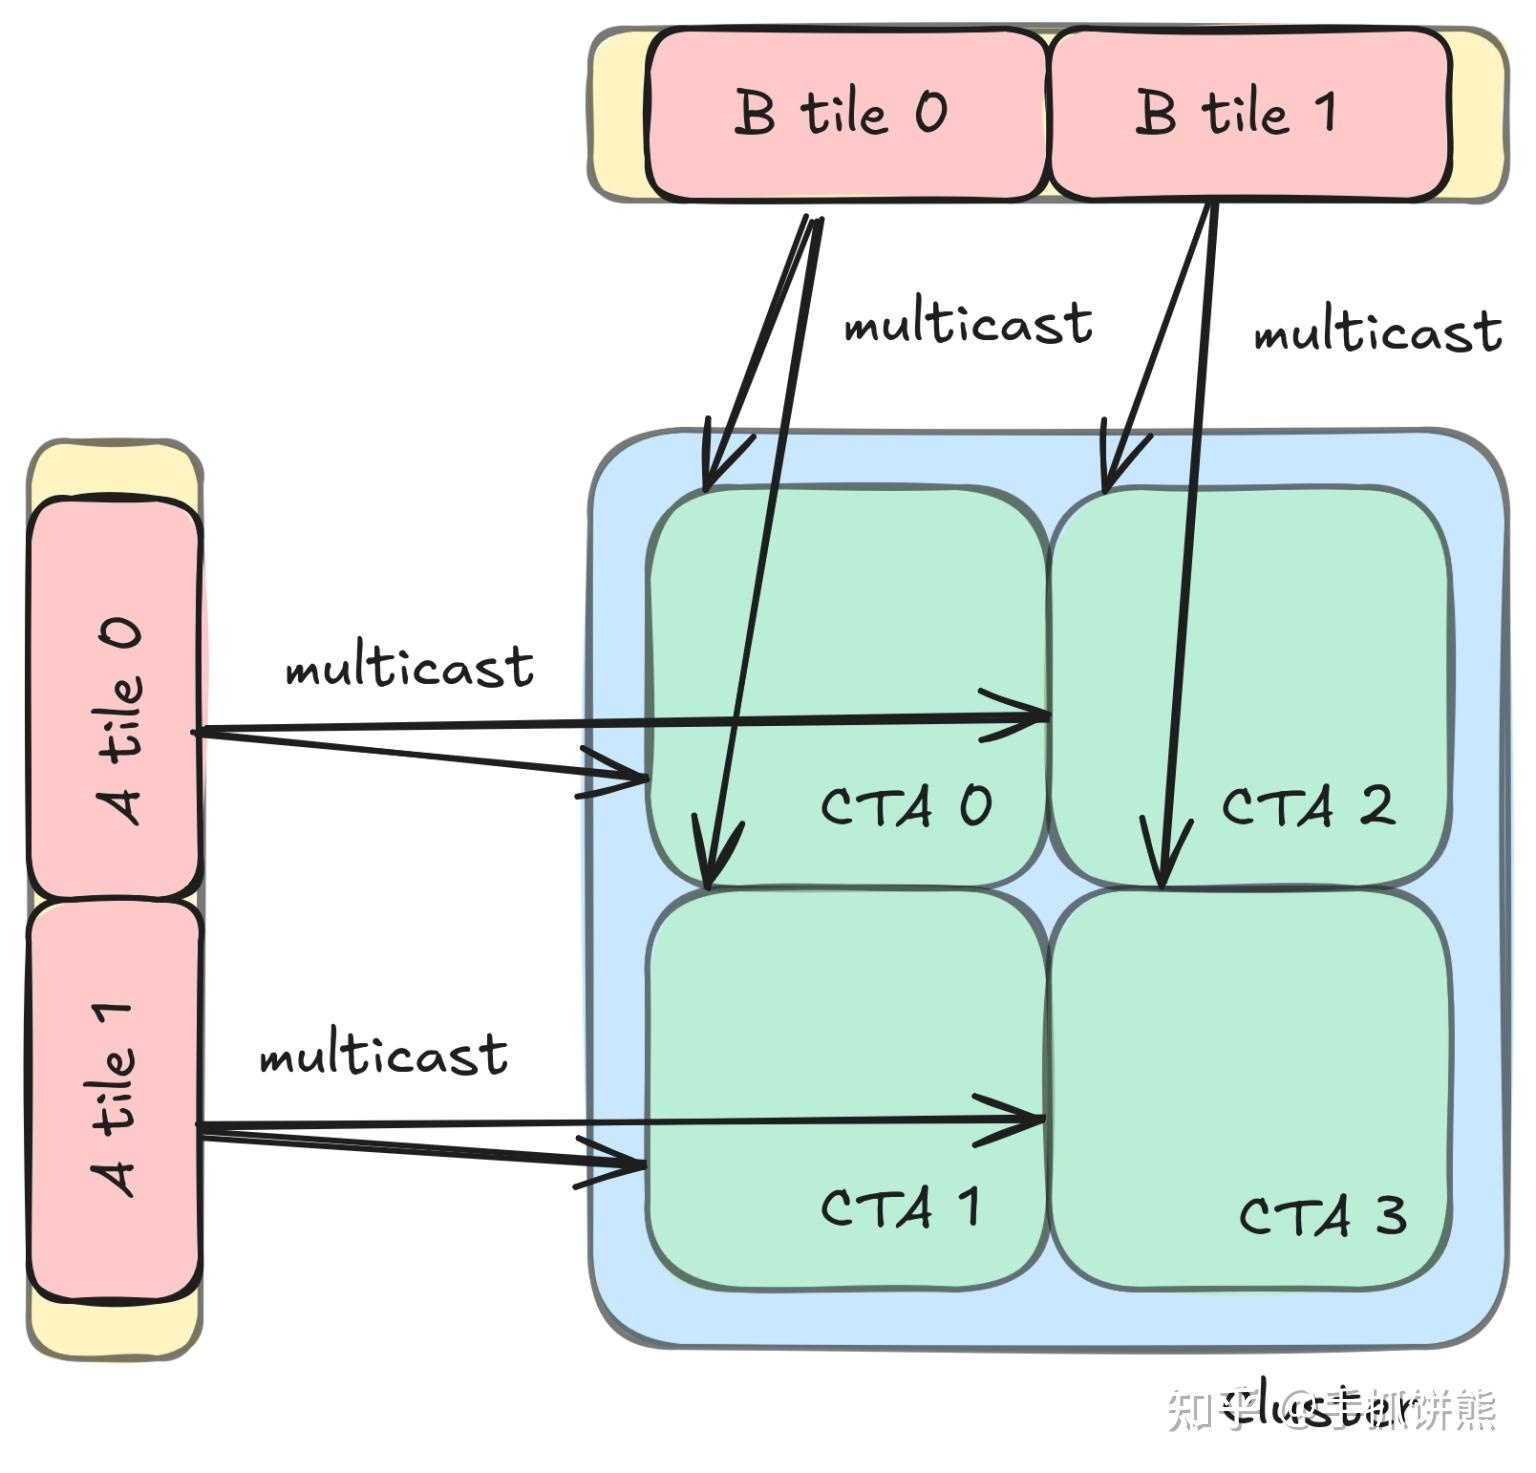
\includegraphics[width=\textwidth]{figures/zhaoshangchun-02-cluster-gemm/fig-03.jpg}
\caption{图 2. 在这个 2×2 cluster中，A 和 B 的每个分片可以使用多播同时加载到 2 个 CTA 中。}
\end{figure}

从概念上讲，TMA 多播相当简单。然而，在实践中，协调多个 CTA 之间的数据访问可能很棘手。因此，可以说 TMA 多播的关键在于正确的同步。从 CTA 工作流程的角度来看，有两个同步点——一个是当所有参与的 TMA 完成且数据准备好供 MMA 使用时，另一个是当所有参与的 MMA 完成且保存数据缓冲区可以被下一次迭代的数据覆盖时。我们将依次讨论这两个点。

\subsection{同步 TMA 参与者}

第一个同步点是等待所有加载所需操作数的 TMA 多播完成。再次强调，对于 A，这是同一行中的所有 CTA；对于 B，这是同一列中的所有 CTA（注意这包括 CTA 自身）。因此，我们需要一个屏障，等待cluster中所有参与相关 TMA 多播操作的 CTA。

为了了解这是如何完成的，让我们看看相关的 PTX。参与信息编码在 \texttt{cp.\allowbreak{}async.\allowbreak{}bulk.\allowbreak{}tensor}（TMA）的 PTX 中：

\begin{figure}[H]\centering
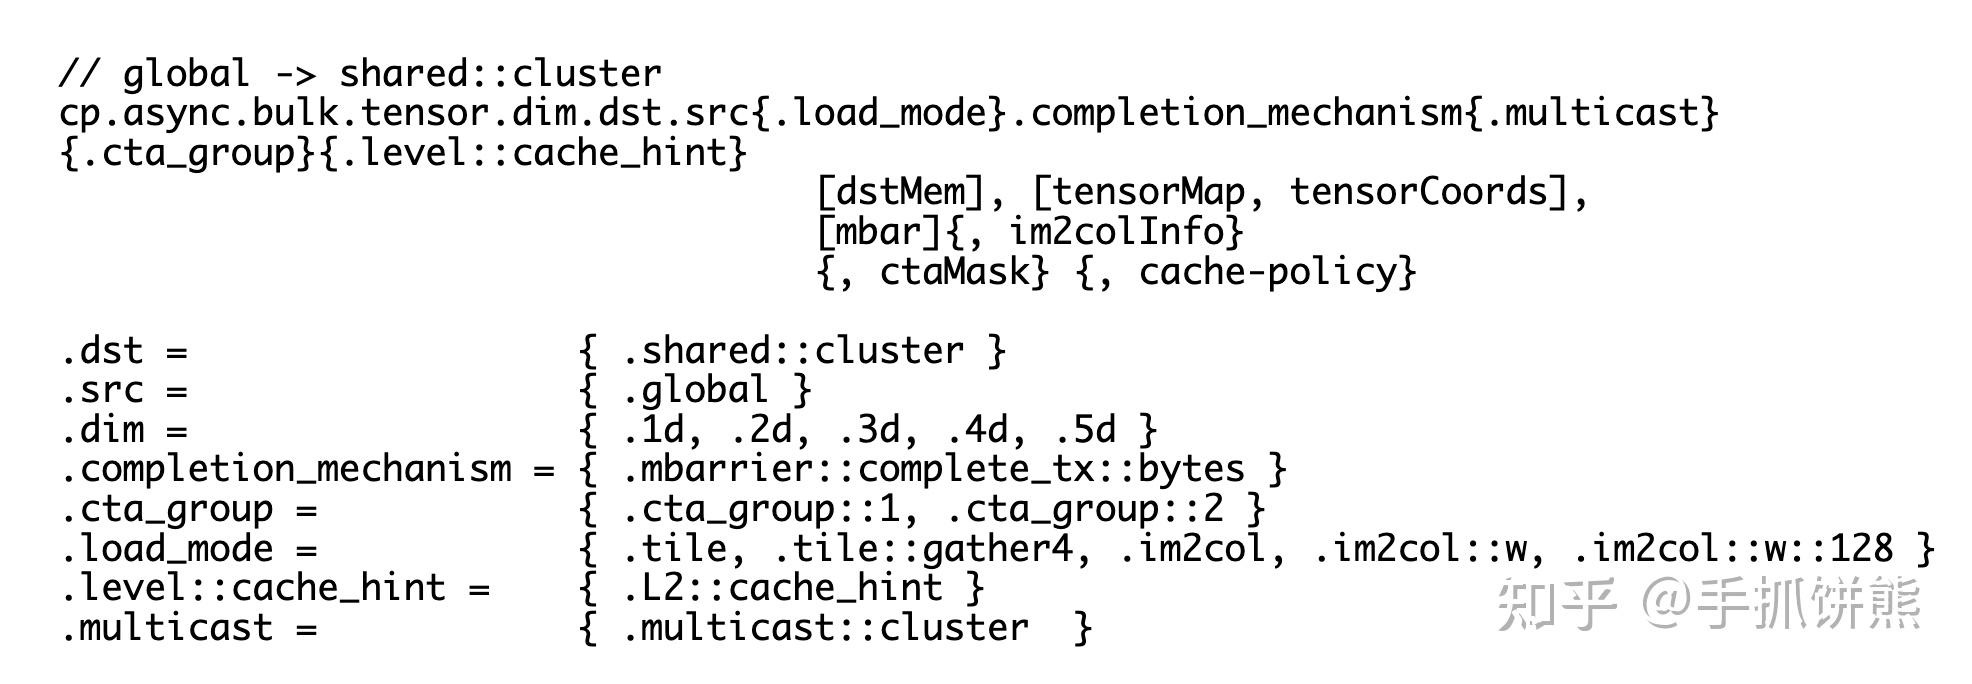
\includegraphics[width=\textwidth]{figures/zhaoshangchun-02-cluster-gemm/fig-04.jpg}
\end{figure}

TMA 多播参与通过 \textbf{\texttt{cta\allowbreak{}Mask}} 指定，它是一个位掩码，第 i 位决定cluster索引为 i 的 CTA 是否参与。更精确地说，TMA 操作将加载的数据放入位掩码指定的所有 CTA 的 SMEM 中，并可选地到达这些 CTA 的 mbarrier。Blackwell GPU 的最大cluster大小为 16，因此我们有一个 16 位的位掩码。对于我们特定的 4x4x1 cluster形状，我们可以通过使用十六进制表示此掩码来获得（相对）易于理解的表达式。例如，cluster索引为 0 的 CTA 具有 \texttt{tma\_\allowbreak{}bitmask\_\allowbreak{}a = 0x1111} 和 \texttt{tma\_\allowbreak{}bitmask\_\allowbreak{}b = 0x000f}。

\begin{figure}[H]\centering
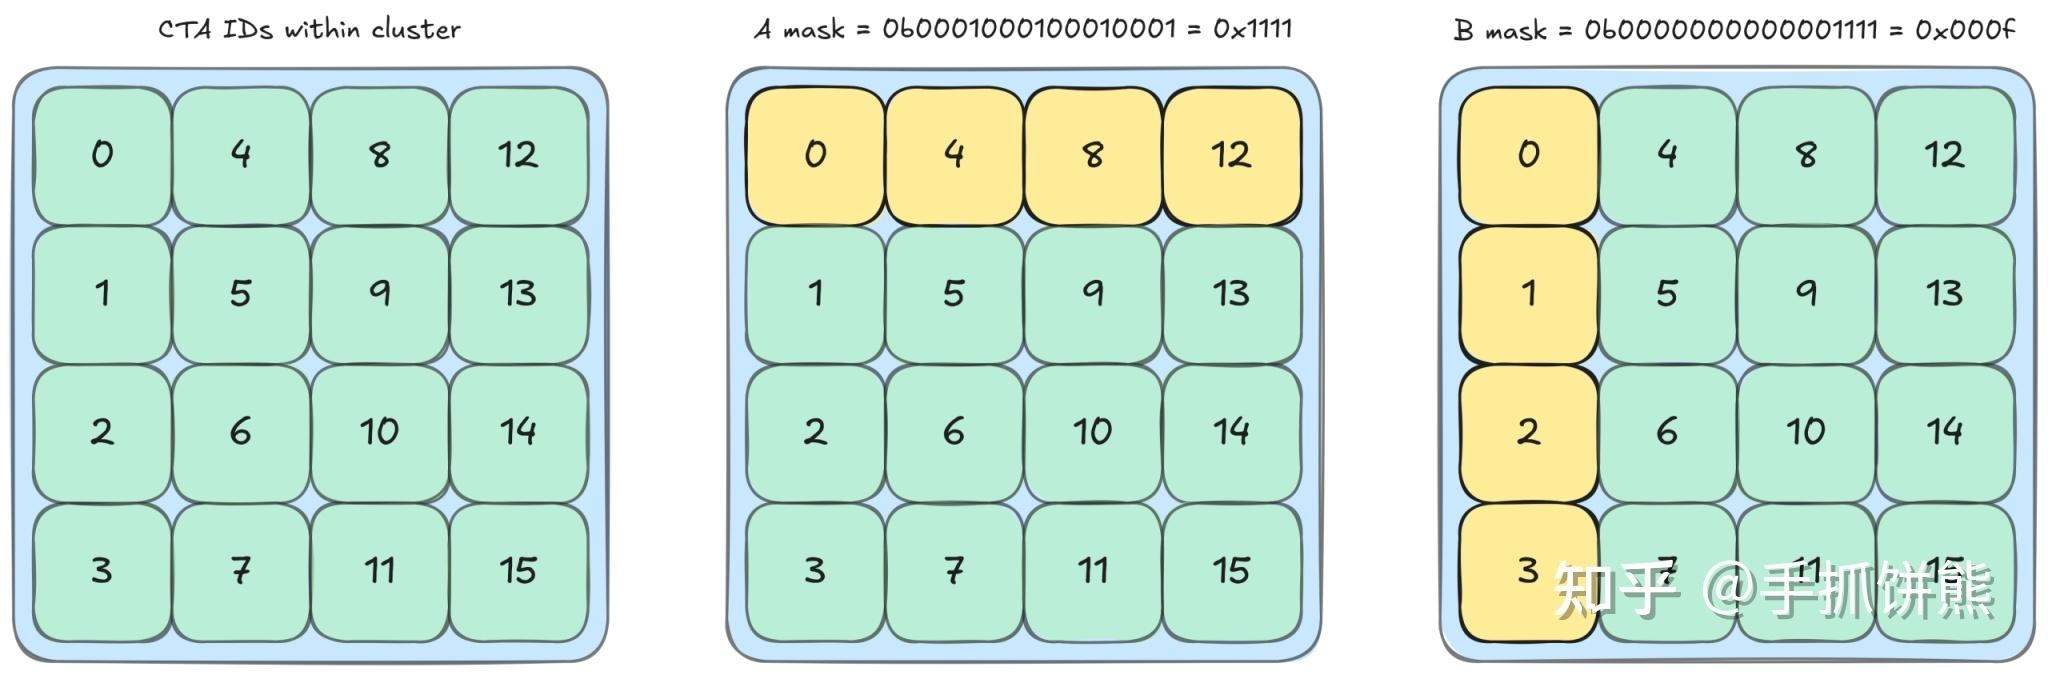
\includegraphics[width=\textwidth]{figures/zhaoshangchun-02-cluster-gemm/fig-05.jpg}
\caption{图 3. cluster内 CTA 的组织，以及与 TMA 索引 0 关联的两个位掩码。请注意，1\allowbreak{}D CTA ID 映射到多维cluster形状，第 0 维是最主要的，这里对应于输出矩阵的 M 维度，因此 CTA 的布局是按列主序的。}
\end{figure}

这里每个位对应一个 CTA，多维cluster形状通过列主序布局映射到一维 CTA 顺序。（cluster中每个 CTA 的一维位置可以通过 PTX 特殊寄存器 \texttt{\%cluster\_\allowbreak{}ctarank} 或使用 \texttt{c\allowbreak{}u\allowbreak{}t\allowbreak{}e\allowbreak{}:\allowbreak{}:\allowbreak{}b\allowbreak{}l\allowbreak{}o\allowbreak{}c\allowbreak{}k\allowbreak{}\_\allowbreak{}r\allowbreak{}a\allowbreak{}n\allowbreak{}k\allowbreak{}\_\allowbreak{}i\allowbreak{}n\allowbreak{}\_\allowbreak{}c\allowbreak{}l\allowbreak{}u\allowbreak{}s\allowbreak{}t\allowbreak{}e\allowbreak{}r\allowbreak{}(\allowbreak{})} 访问。）我们可以看到列和行的参与是如何编码在掩码中的：例如，在 A 的位掩码中，CTA 0 与 CTA 4、8 和 12 共享同一行，因此掩码 \texttt{0b0001000100010001} 在位 0、4、8 和 12 处为 1。使用此掩码，由 CTA 0 发出的 TMA 多播操作将把加载的数据放入 CTA 0、4、8 和 12 的 SMEM 中，并到达它们各自的 mbarrier。同一行的 CTA 对 A 发出的 TMA 多播都使用相同的位掩码（对于顶行是 \texttt{0x1111}），同一列的 CTA 对 B 发出的 TMA 多播都使用相同的位掩码（对于最左列是 \texttt{0x000f}）。这使得 CTA 只需等待参与其操作数多播加载的其他 6 个 CTA。

现在让我们看看这个 TMA 多播和同步在示例中是如何实现的。首先是拷贝原子。对于这种简单的单 SM 情况，示例使用了 \texttt{sm90} TMA 原子。参数与标准 TMA 相同，只是附加了多播模式中的 CTA 数量。请注意，多播模式（给出参与者数量）对于 A 被选择为 N 维（其中 A 是 Mx\allowbreak{}K）。

\begin{figure}[H]\centering
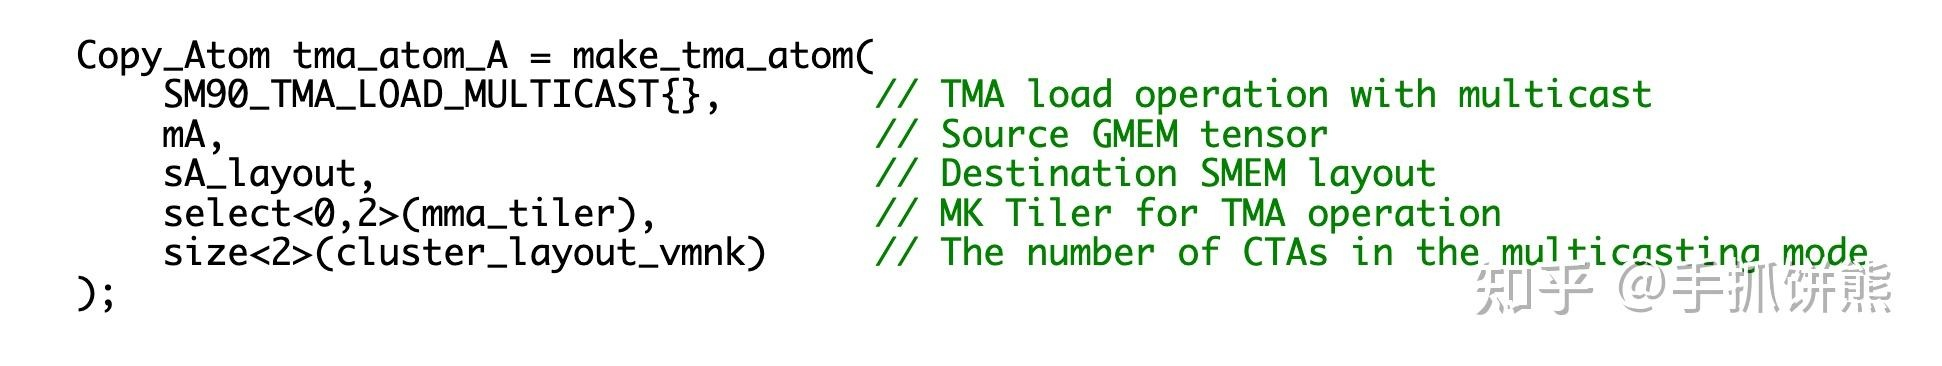
\includegraphics[width=\textwidth]{figures/zhaoshangchun-02-cluster-gemm/fig-06.jpg}
\end{figure}

接下来，要启动 TMA 多播，我们需要位掩码。这个位掩码可以通过 CUTLASS 的一个实用函数构造：

\begin{figure}[H]\centering
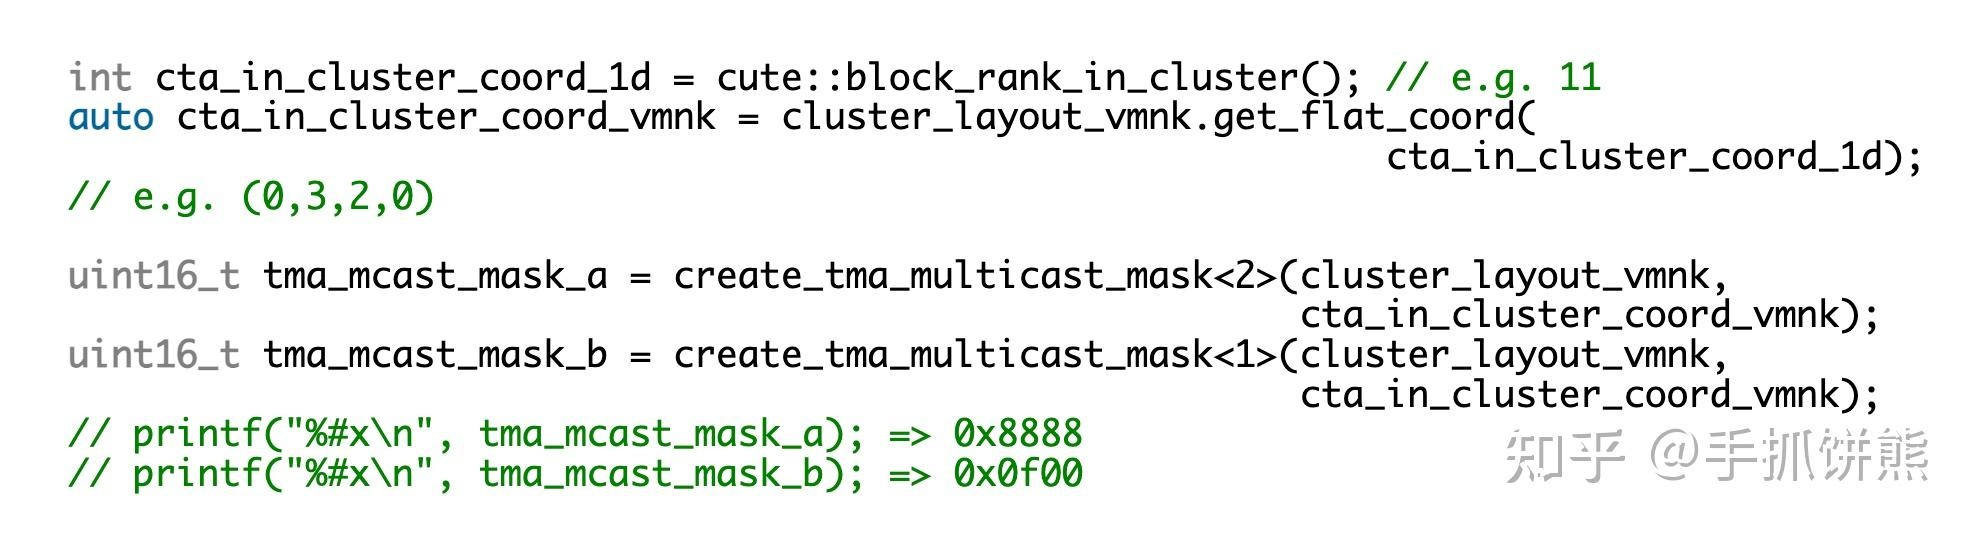
\includegraphics[width=\textwidth]{figures/zhaoshangchun-02-cluster-gemm/fig-07.jpg}
\end{figure}

TMA 多播所需的最后一组信息是数据张量。我们可以使用 TMA 分区器来获取分区后的分片：

\begin{figure}[H]\centering
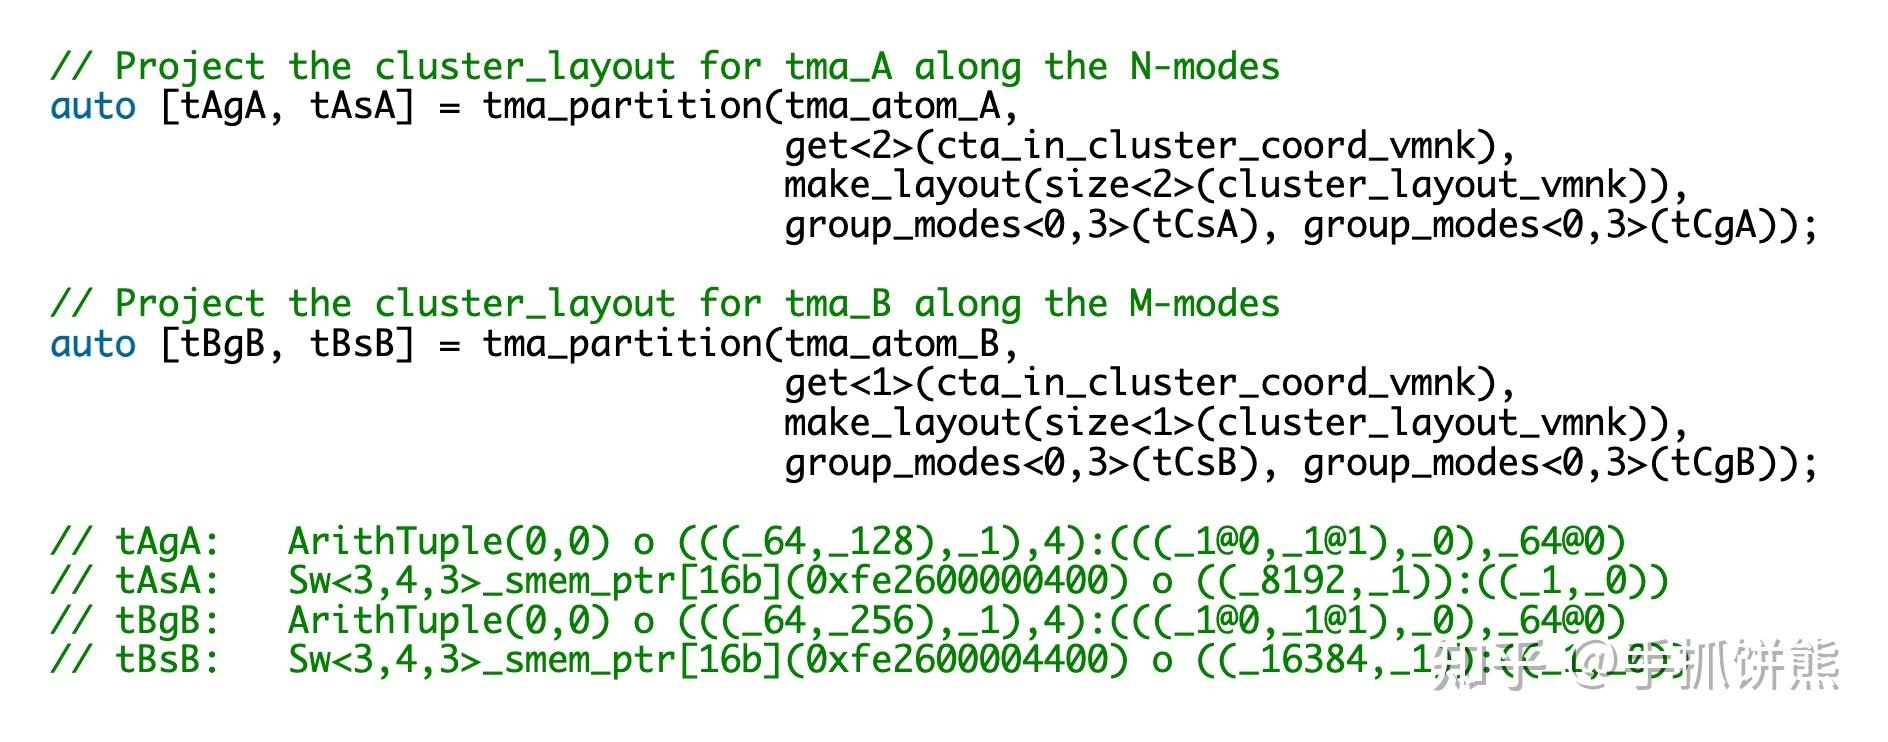
\includegraphics[width=\textwidth]{figures/zhaoshangchun-02-cluster-gemm/fig-08.jpg}
\end{figure}

这里一个有趣的点是，尽管每个 CTA 负责从 GMEM 加载共享分片的一个切片，但这里显示的分区后张量显示了整个分片。实际上，这些张量与常规 TMA 的张量看起来相同。这是因为关于 TMA 多播切片的信息是通过内存地址偏移量传递的，该偏移量存储在 \texttt{Arith\allowbreak{}Tuple(0,\allowbreak{}0)} 中。但由于此打印输出是在 CTA 0 上生成的，所以偏移量为零。我们可以通过查看 CTA 1 的 \texttt{t\allowbreak{}Ag\allowbreak{}A} 来看到这个偏移量：

\begin{figure}[H]\centering
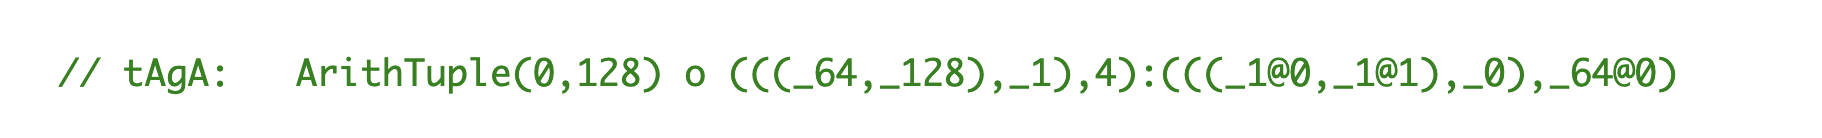
\includegraphics[width=\textwidth]{figures/zhaoshangchun-02-cluster-gemm/fig-09.png}
\end{figure}

每个 CTA 接收整个分片的相同布局，但不同的内存偏移量指示它们要拷贝数据的哪个切片。更深入的讨论，请参考我们之前关于 TMA 的博客文章。

我们现在拥有了启动 TMA 多播和同步所需的所有信息。除了参数中的位掩码外，TMA 启动本身与我们之前介绍过的标准 TMA 启动相同：

\begin{figure}[H]\centering
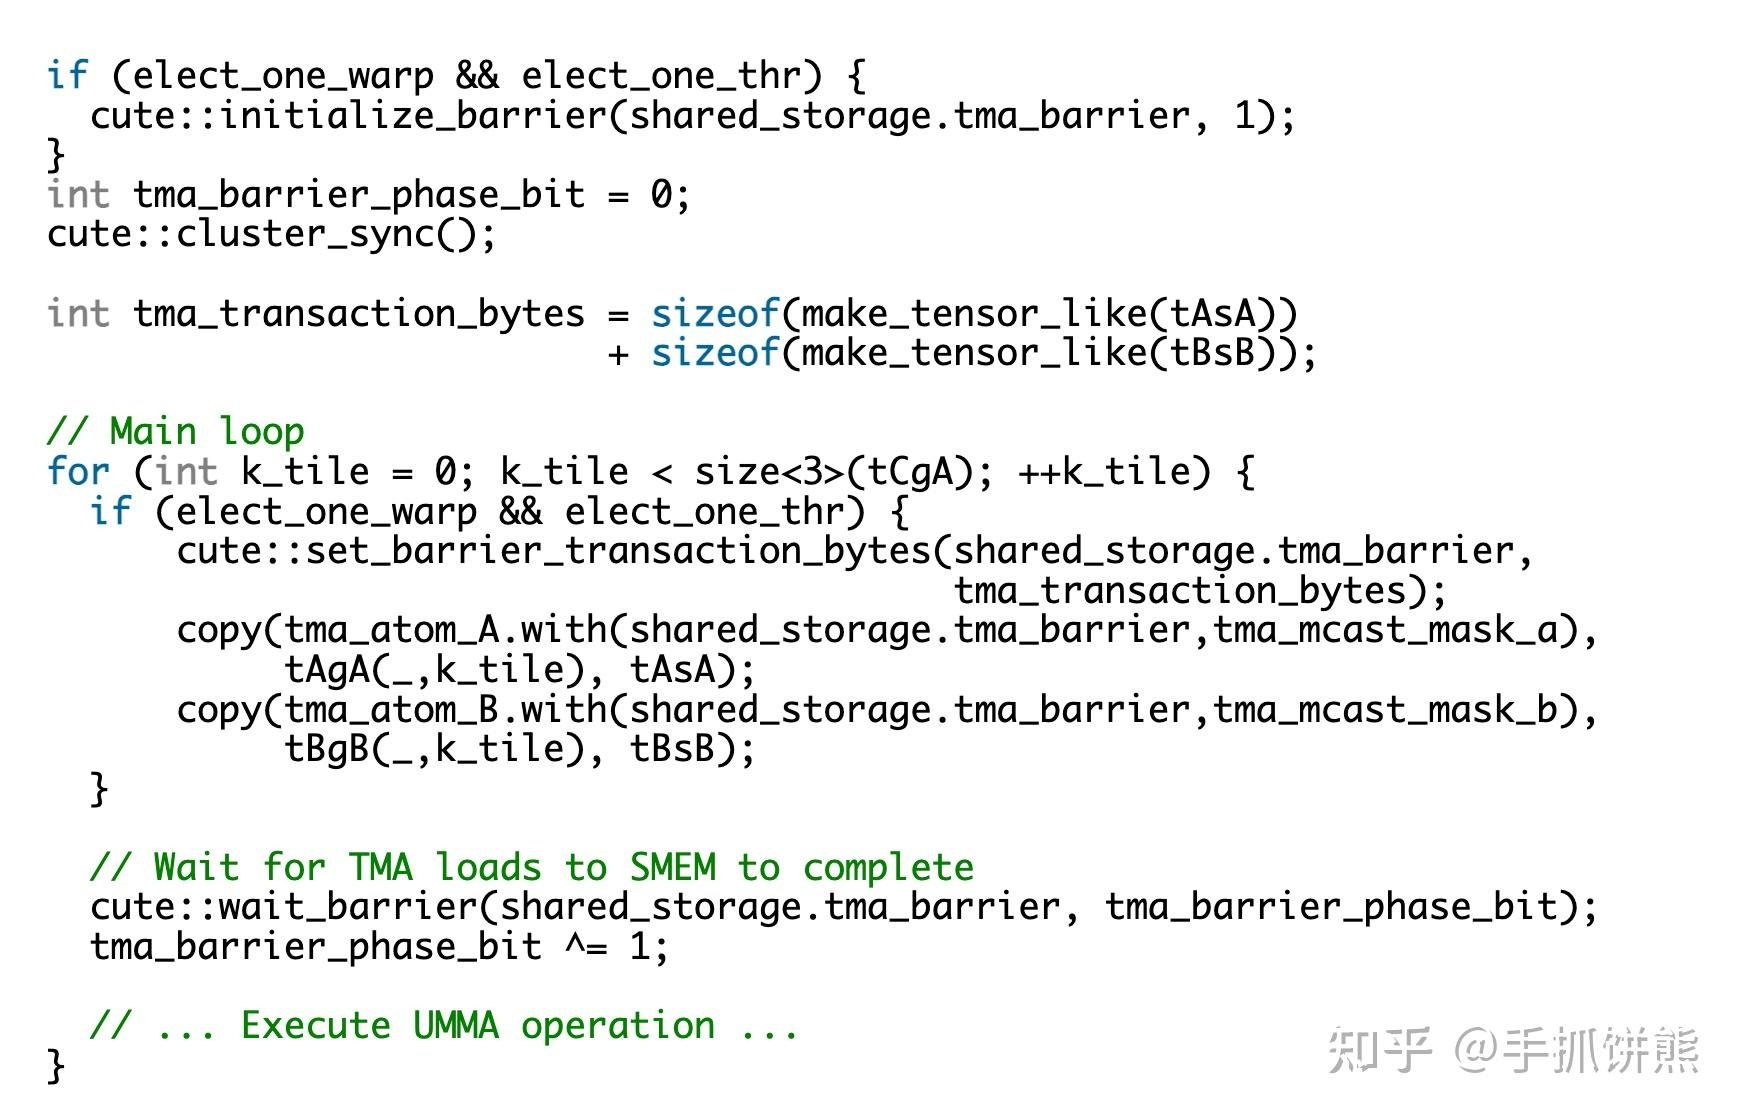
\includegraphics[width=\textwidth]{figures/zhaoshangchun-02-cluster-gemm/fig-10.jpg}
\end{figure}

这里需要注意的重要一点是 TMA 屏障完成以及 \texttt{transaction\_\allowbreak{}bytes} 的值。\texttt{mbarrier} 对象有两个内部计数器，用于跟踪当前阶段的完成情况：一个线程中的待处理到达计数和一个待处理事务计数（tx-count，以字节为单位）。当两个计数都达到 0 时，该阶段完成。这里感兴趣的主要计数是 tx-count，它通过 \texttt{c\allowbreak{}u\allowbreak{}t\allowbreak{}e\allowbreak{}:\allowbreak{}:\allowbreak{}s\allowbreak{}e\allowbreak{}t\allowbreak{}\_\allowbreak{}b\allowbreak{}a\allowbreak{}r\allowbreak{}r\allowbreak{}i\allowbreak{}e\allowbreak{}r\allowbreak{}\_\allowbreak{}t\allowbreak{}r\allowbreak{}a\allowbreak{}n\allowbreak{}s\allowbreak{}a\allowbreak{}c\allowbreak{}t\allowbreak{}i\allowbreak{}o\allowbreak{}n\allowbreak{}\_\allowbreak{}b\allowbreak{}y\allowbreak{}t\allowbreak{}e\allowbreak{}s} 设置为预期的 TMA 加载大小。（顺便提一下，此函数内部调用 \texttt{m\allowbreak{}b\allowbreak{}a\allowbreak{}r\allowbreak{}r\allowbreak{}i\allowbreak{}e\allowbreak{}r\allowbreak{}.\allowbreak{}a\allowbreak{}r\allowbreak{}r\allowbreak{}i\allowbreak{}v\allowbreak{}e\allowbreak{}.\allowbreak{}e\allowbreak{}x\allowbreak{}p\allowbreak{}e\allowbreak{}c\allowbreak{}t\allowbreak{}\_\allowbreak{}t\allowbreak{}x}，它消耗了初始化中设置的 1 个到达计数。）到达时，TMA 拷贝会将 mbarrier 的 tx-count 减少拷贝的数据字节数。我们将其设置为操作数分片的总大小，因为在继续执行 UMMA 之前，我们需要等待所有操作数数据被参与的 CTA 加载完毕。

\subsection{UMMA 后同步}

此处的 UMMA 与上一篇文章中看到的相同，因此我们将重点放在屏障同步上。UMMA 是一个异步操作，因此我们必须显式等待它完成。在前面的示例中，我们只需要等待执行 CTA 完成 MMA，然后再继续下一次迭代。但是，这里我们还需要确保其他 CTA 在通过多播覆盖操作数数据之前，已完成对 SMEM 中操作数数据的消耗。换句话说，每个 CTA 需要等待自身以及与它共享操作数数据的所有其他 CTA 完成它们的 MMA，然后才能发出下一次 TMA 加载。

一个简单的解决方案是直接添加 \texttt{cute::\allowbreak{}cluster\_\allowbreak{}sync()} 并确保cluster中的所有 CTA 在继续之前都已完成。但我们可以做得更好；\texttt{cluster\_\allowbreak{}sync()} 有些过度，因为对于给定的分片，并非所有 CTA 都在其 GEMM 中使用它。相反，每个 CTA 应该只等待与其共享 A 分片的另外 3 个 CTA，以及与其共享 B 分片的另外 3 个 CTA。这种有针对性的同步将允许cluster中的某些 CTA 提前运行并发出 TMA 加载，而其他 CTA 仍在完成其 MMA 操作。

这种子cluster级别的同步与我们为 TMA 多播看到的类似。但由于它现在与异步张量核心操作的完成相关联，它使用了一些 Blackwell 新增的指令，特别是 \textbf{\texttt{tcgen05.\allowbreak{}commit}} 指令或其 CUTLASS 包装器 \textbf{\texttt{c\allowbreak{}u\allowbreak{}t\allowbreak{}l\allowbreak{}a\allowbreak{}s\allowbreak{}s\allowbreak{}:\allowbreak{}:\allowbreak{}a\allowbreak{}r\allowbreak{}c\allowbreak{}h\allowbreak{}:\allowbreak{}:\allowbreak{}u\allowbreak{}m\allowbreak{}m\allowbreak{}a\allowbreak{}\_\allowbreak{}a\allowbreak{}r\allowbreak{}r\allowbreak{}i\allowbreak{}v\allowbreak{}e\allowbreak{}\_\allowbreak{}m\allowbreak{}u\allowbreak{}l\allowbreak{}t\allowbreak{}i\allowbreak{}c\allowbreak{}a\allowbreak{}s\allowbreak{}t}}。该指令将之前的异步 \texttt{tcgen05} 操作（如 UMMA）分组，并指示它们在完成时到达其cluster中某些 CTA 的共享内存空间中的 mbarrier，这些 CTA 由位掩码指定。

因此，我们将设置一个类似于我们为 TMA 创建的带位掩码的同步。这次，我们需要一个掩码来编码哪些其他 CTA 正在使用该 CTA 已加载的分片。要构造这个掩码，我们可以使用之前创建的 TMA 位掩码。A 的位掩码告诉我们哪些其他 CTA 正在使用 A 操作数，B 的位掩码也是如此。因此，我们可以通过取两个掩码的按位 OR 来获得所需的位掩码。例如，对于cluster中索引为 0 的 CTA，我们发现 TMA 位掩码为 \texttt{tma\_\allowbreak{}bitmask\_\allowbreak{}a = 0x1111} 和 \texttt{tma\_\allowbreak{}bitmask\_\allowbreak{}b = 0x000f}。所以 MMA 位掩码是 \texttt{t\allowbreak{}m\allowbreak{}a\allowbreak{}\_\allowbreak{}b\allowbreak{}i\allowbreak{}t\allowbreak{}m\allowbreak{}a\allowbreak{}s\allowbreak{}k\allowbreak{}\_\allowbreak{}a\allowbreak{}|\allowbreak{}t\allowbreak{}m\allowbreak{}a\allowbreak{}\_\allowbreak{}b\allowbreak{}i\allowbreak{}t\allowbreak{}m\allowbreak{}a\allowbreak{}s\allowbreak{}k\allowbreak{}\_\allowbreak{}b\allowbreak{} \allowbreak{}=\allowbreak{} \allowbreak{}0\allowbreak{}x\allowbreak{}1\allowbreak{}1\allowbreak{}1\allowbreak{}f}。

\begin{figure}[H]\centering
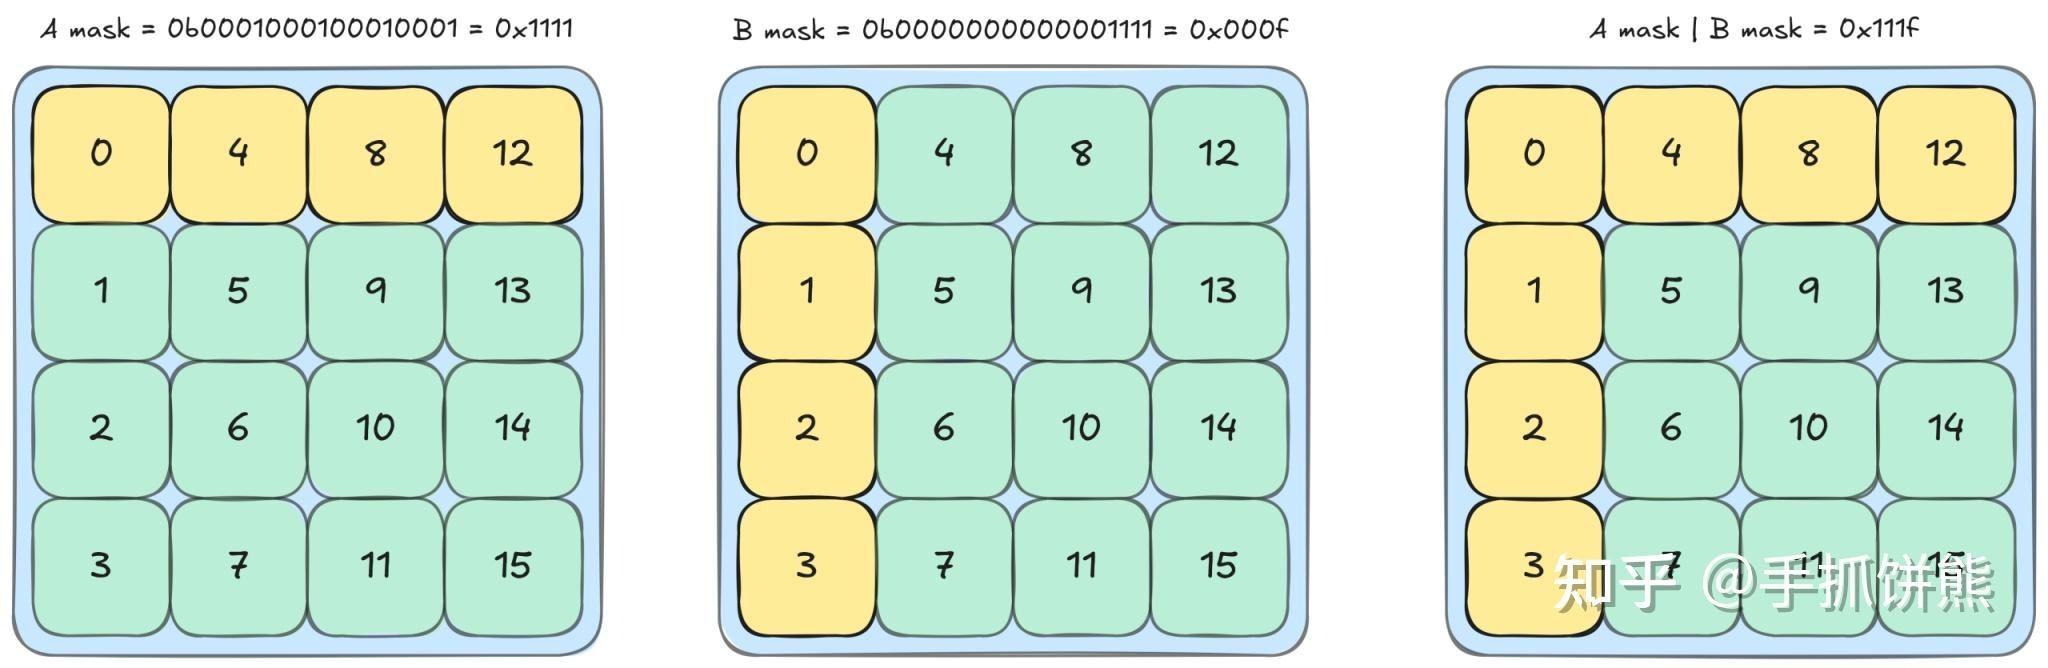
\includegraphics[width=\textwidth]{figures/zhaoshangchun-02-cluster-gemm/fig-11.jpg}
\caption{图 4. MMA 位掩码是 TMA 位掩码的按位 OR。右侧是 CTA 0 的 MMA 位掩码。}
\end{figure}

在图中我们可以看到，这个位掩码标识了与 CTA 0 共享一个分片的 CTA，即同一列或同一行的 CTA。

有了这个位掩码，我们就可以设置 MMA 同步了。第一步，mbarrier 的创建，与 TMA 情况有一个关键区别——因为没有数据传输，我们依赖到达计数而不是 tx-count。具体来说，屏障计数需要设置为等于参与的 MMA 数量。在此示例中，每个 CTA 的屏障需要等待 7 个线程；这计数了从掩码中出现的所有 CTA 发出 MMA 的所有线程，包括自身。更一般地，这个数字可以从cluster布局中获取，确保避免重复计算自身。

\begin{figure}[H]\centering
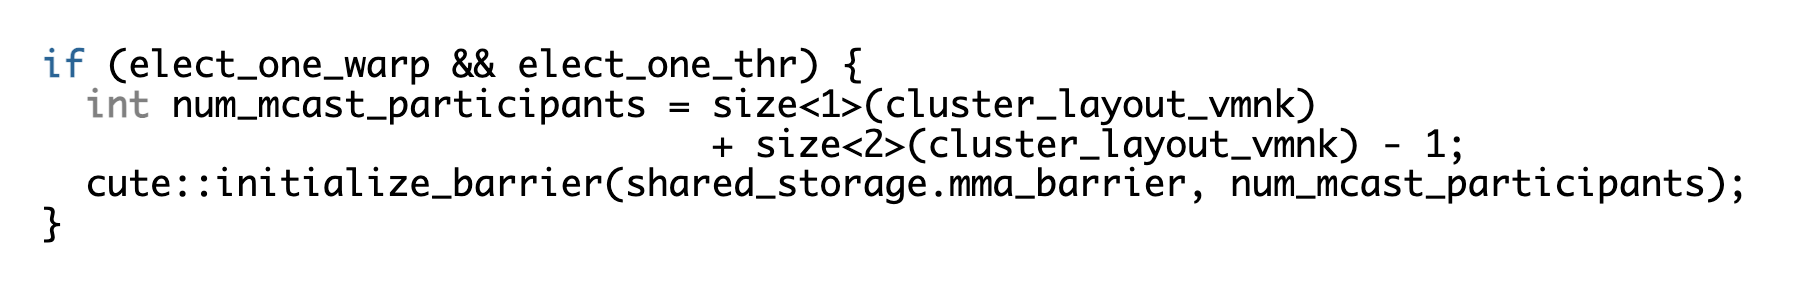
\includegraphics[width=\textwidth]{figures/zhaoshangchun-02-cluster-gemm/fig-12.png}
\end{figure}

最后，我们可以设置同步。我们将发出 \texttt{tcgen05.\allowbreak{}mma} 的内部循环与 \texttt{umma\_\allowbreak{}arrive\_\allowbreak{}multicast} 组合在一起，并指示它在完成时到达位掩码指定的 CTA 的 mbarrier。

\begin{figure}[H]\centering
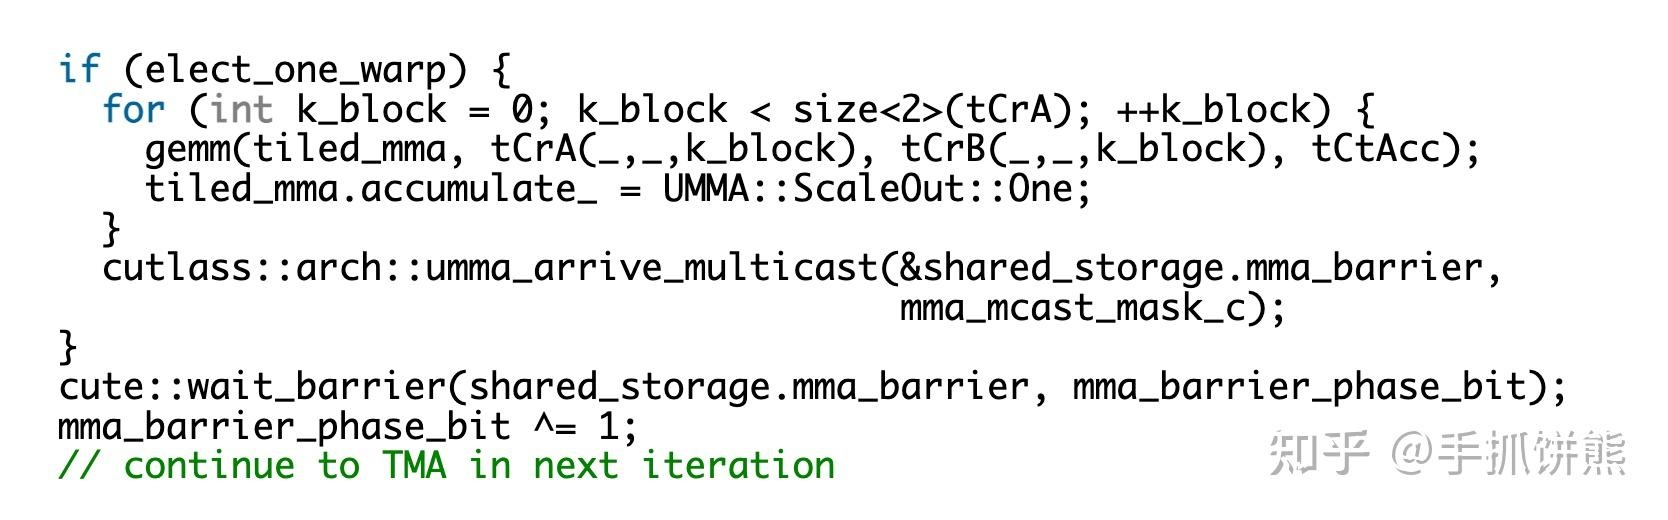
\includegraphics[width=\textwidth]{figures/zhaoshangchun-02-cluster-gemm/fig-13.jpg}
\end{figure}

注意 \texttt{umma\_\allowbreak{}arrive\_\allowbreak{}multicast} 内部会选择单个线程到达屏障，因此我们不应像对 TMA 设置事务计数那样显式选择一个线程。有了这个有针对性的屏障，CTA 可以继续执行，而不必等待cluster中的所有 CTA——只需等待那些有数据依赖关系的 CTA。即使cluster中的某些其他 CTA 仍在计算 MMA，它也能够启动下一次 k 迭代的 TMA。

\section{CuTe 示例：使用 TMA 多播的 Pair-UMMA}

接下来，让我们检查示例 4，在这里我们遇到了 2 SM 的情况。回顾上一篇文章，Blackwell 增加了同一cluster中两个相邻 CTA 协同处理 UMMA 的能力。据我们所知，这种 MMA 变体没有正式名称，因此我们将其称为 \textbf{2-SM UMMA} 或 \textbf{pair-UMMA}。同样，当需要澄清时，我们将使用术语 \textbf{1-SM UMMA} 或 \textbf{single-UMMA}。

Pair-UMMA 为索引增加了一层复杂性，因为现在我们需要区分 MMA 坐标和 CTA 坐标。以前，每个 CTA 在每个主循环迭代中计算一个 \texttt{(b\allowbreak{}M,\allowbreak{} b\allowbreak{}N,\allowbreak{} b\allowbreak{}K)} MMA 操作。因此，CTA 自然地排列在三维网格中。随着 Pair-UMMA 的引入，现在更好地将其视为 \texttt{(b\allowbreak{}M,\allowbreak{} b\allowbreak{}N,\allowbreak{} b\allowbreak{}K)} MMA 分片的网格，其中一个 MMA 分片可能由 1 个或 2 个 CTA 组成的 CTA 组计算。这意味着最好将 CTA 视为位于一个四维网格上，其中第 0 个“值”模式表示 CTA 在其组内的索引。请注意，这个概念步骤实际上不受 CUDA 语法支持，CUDA 仅使用三维网格形状，因此必须手动对 CTA 索引进行一些算术运算。

在本节中，我们将首先更深入地研究考虑 CTA 对时的两种索引方案。然后，我们将浏览示例并讨论 pair-UMMA 如何改变索引和分区。最后，一旦我们知道每个 CTA 需要哪些数据，我们将研究 CTA 对如何改变我们应该使用 TMA 的方式。

\subsection{用于 CTA 对的线程块cluster}

CTA 对必须位于单个cluster中，并且cluster内的 CTA 使用cluster内的 CTA ID 进行配对。具体来说，索引的第 0 位不同的 CTA（例如 0 和 1、2 和 3 等）被视为一对。在对中，索引为偶数的 CTA 称为\textbf{偶数 CTA}，索引为奇数的 CTA 称为\textbf{奇数 CTA}。

现在考虑形状为 \texttt{<4,\allowbreak{}4,\allowbreak{}1>} 的cluster，它有 8 对。由于这是 Cu\allowbreak{}Te，此形状在索引上是列主序的；因此配对发生在最左边的模式上，其大小至少为 2。对于 \texttt{<4,\allowbreak{}4,\allowbreak{}1>}，这意味着第 0 个模式决定了配对。请注意，配对模式的选择可能受到特定张量核心操作的限制；例如，pair-UMMA 要求配对在 M 模式上进行。

让我们回顾一下上一篇文章中简要介绍的 \texttt{cluster\_\allowbreak{}shape\_\allowbreak{}vmnk}。

\begin{figure}[H]\centering
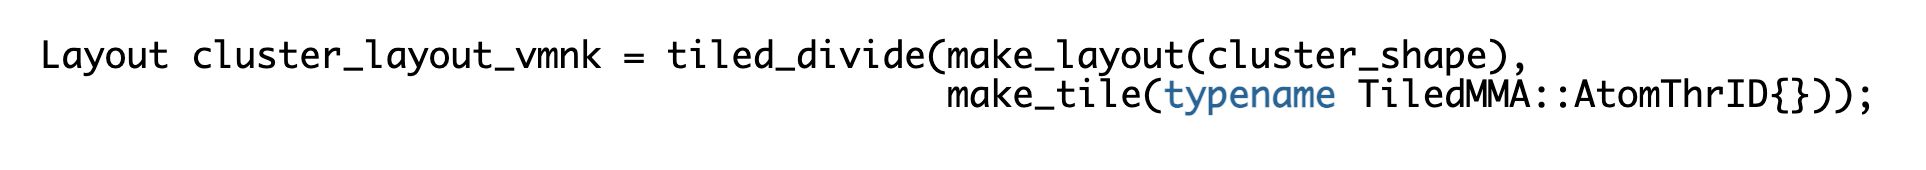
\includegraphics[width=\textwidth]{figures/zhaoshangchun-02-cluster-gemm/fig-14.png}
\end{figure}

我们看到，当使用 single-UMMA 时，\texttt{Atom\allowbreak{}Thr\allowbreak{}ID\{\}} 的值为 1，并且 \texttt{cluster\_\allowbreak{}layout\_\allowbreak{}vmnk} 简化为 \texttt{<\allowbreak{}1\allowbreak{},\allowbreak{}c\allowbreak{}l\allowbreak{}u\allowbreak{}s\allowbreak{}t\allowbreak{}e\allowbreak{}r\allowbreak{}.\allowbreak{}x\allowbreak{},\allowbreak{}c\allowbreak{}l\allowbreak{}u\allowbreak{}s\allowbreak{}t\allowbreak{}e\allowbreak{}r\allowbreak{}.\allowbreak{}y\allowbreak{},\allowbreak{}c\allowbreak{}l\allowbreak{}u\allowbreak{}s\allowbreak{}t\allowbreak{}e\allowbreak{}r\allowbreak{}.\allowbreak{}z\allowbreak{}>}。但现在我们有了 pair-UMMA 原子，所以 \texttt{Atom\allowbreak{}Thr\allowbreak{}ID\{\}} 是 2。因此，此处的 \texttt{tiled\_\allowbreak{}divide} 将沿着cluster形状的第 0 维用大小为 (2) 的分片进行平铺，从而为 CTA cluster创建一个秩为 4 的布局。同样，第 0 个“值”模式将决定对内的 ID，其他三个模式构成cluster中 CTA 对的布局。例如，对于形状为 \texttt{<4,\allowbreak{}4,\allowbreak{}1>} 的cluster：

\begin{figure}[H]\centering
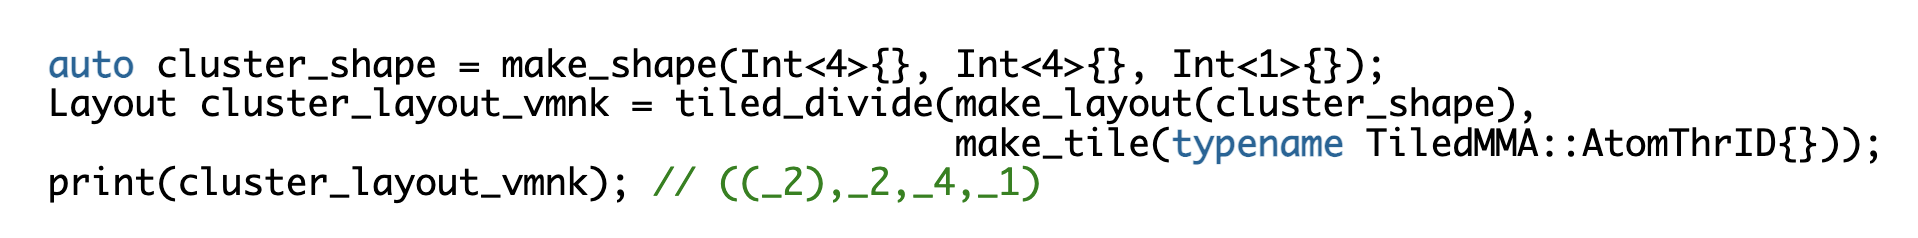
\includegraphics[width=\textwidth]{figures/zhaoshangchun-02-cluster-gemm/fig-15.png}
\end{figure}

我们可以将其解读为 8 个 CTA 对排列成 \texttt{(2,\allowbreak{}4,\allowbreak{}1)} 的形状。然后，这个cluster布局用于计算 \texttt{mma\_\allowbreak{}coord\_\allowbreak{}vmnk}。

\begin{figure}[H]\centering
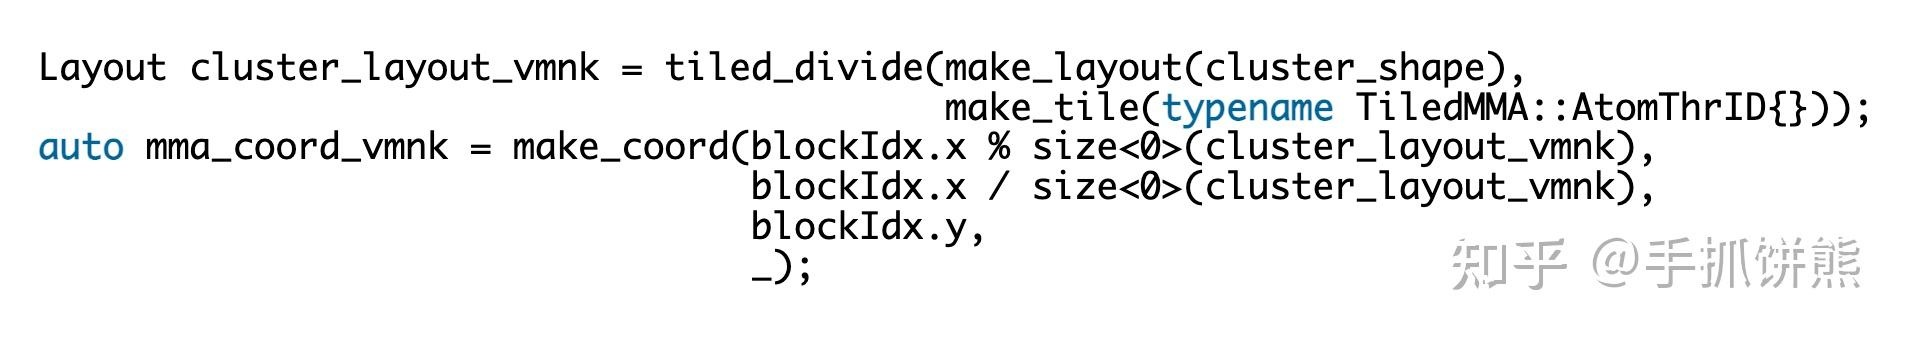
\includegraphics[width=\textwidth]{figures/zhaoshangchun-02-cluster-gemm/fig-16.jpg}
\end{figure}

\texttt{mma\_\allowbreak{}coord\_\allowbreak{}vmnk} 有点像一个复合坐标系；第 0 个模式是单个 MMA 内部的对等 CTA 坐标，而模式 1 到 3 是 MMA 的全局坐标。后三个模式组成了 MMA 坐标，这些坐标用于索引 MMA 分片。Blackwell 架构的 MMA 是\textbf{对本地}的，而 Hopper 架构中它是 CTA 本地的。

\subsection{Pair-UMMA}

在 pair-UMMA 中，对中的 CTA 协同处理同一个 MMA 分片。对中的每个 CTA 加载每个 MMA 操作数分片的一半，并在其 TMEM 中保存一半的累加器。例如，如果 MMA 是 256x256x16，那么每个 CTA 从 A 和 B 加载 128×16 的切片，并在 TMEM 中保存一个 128×256 的累加器矩阵。

\begin{figure}[H]\centering
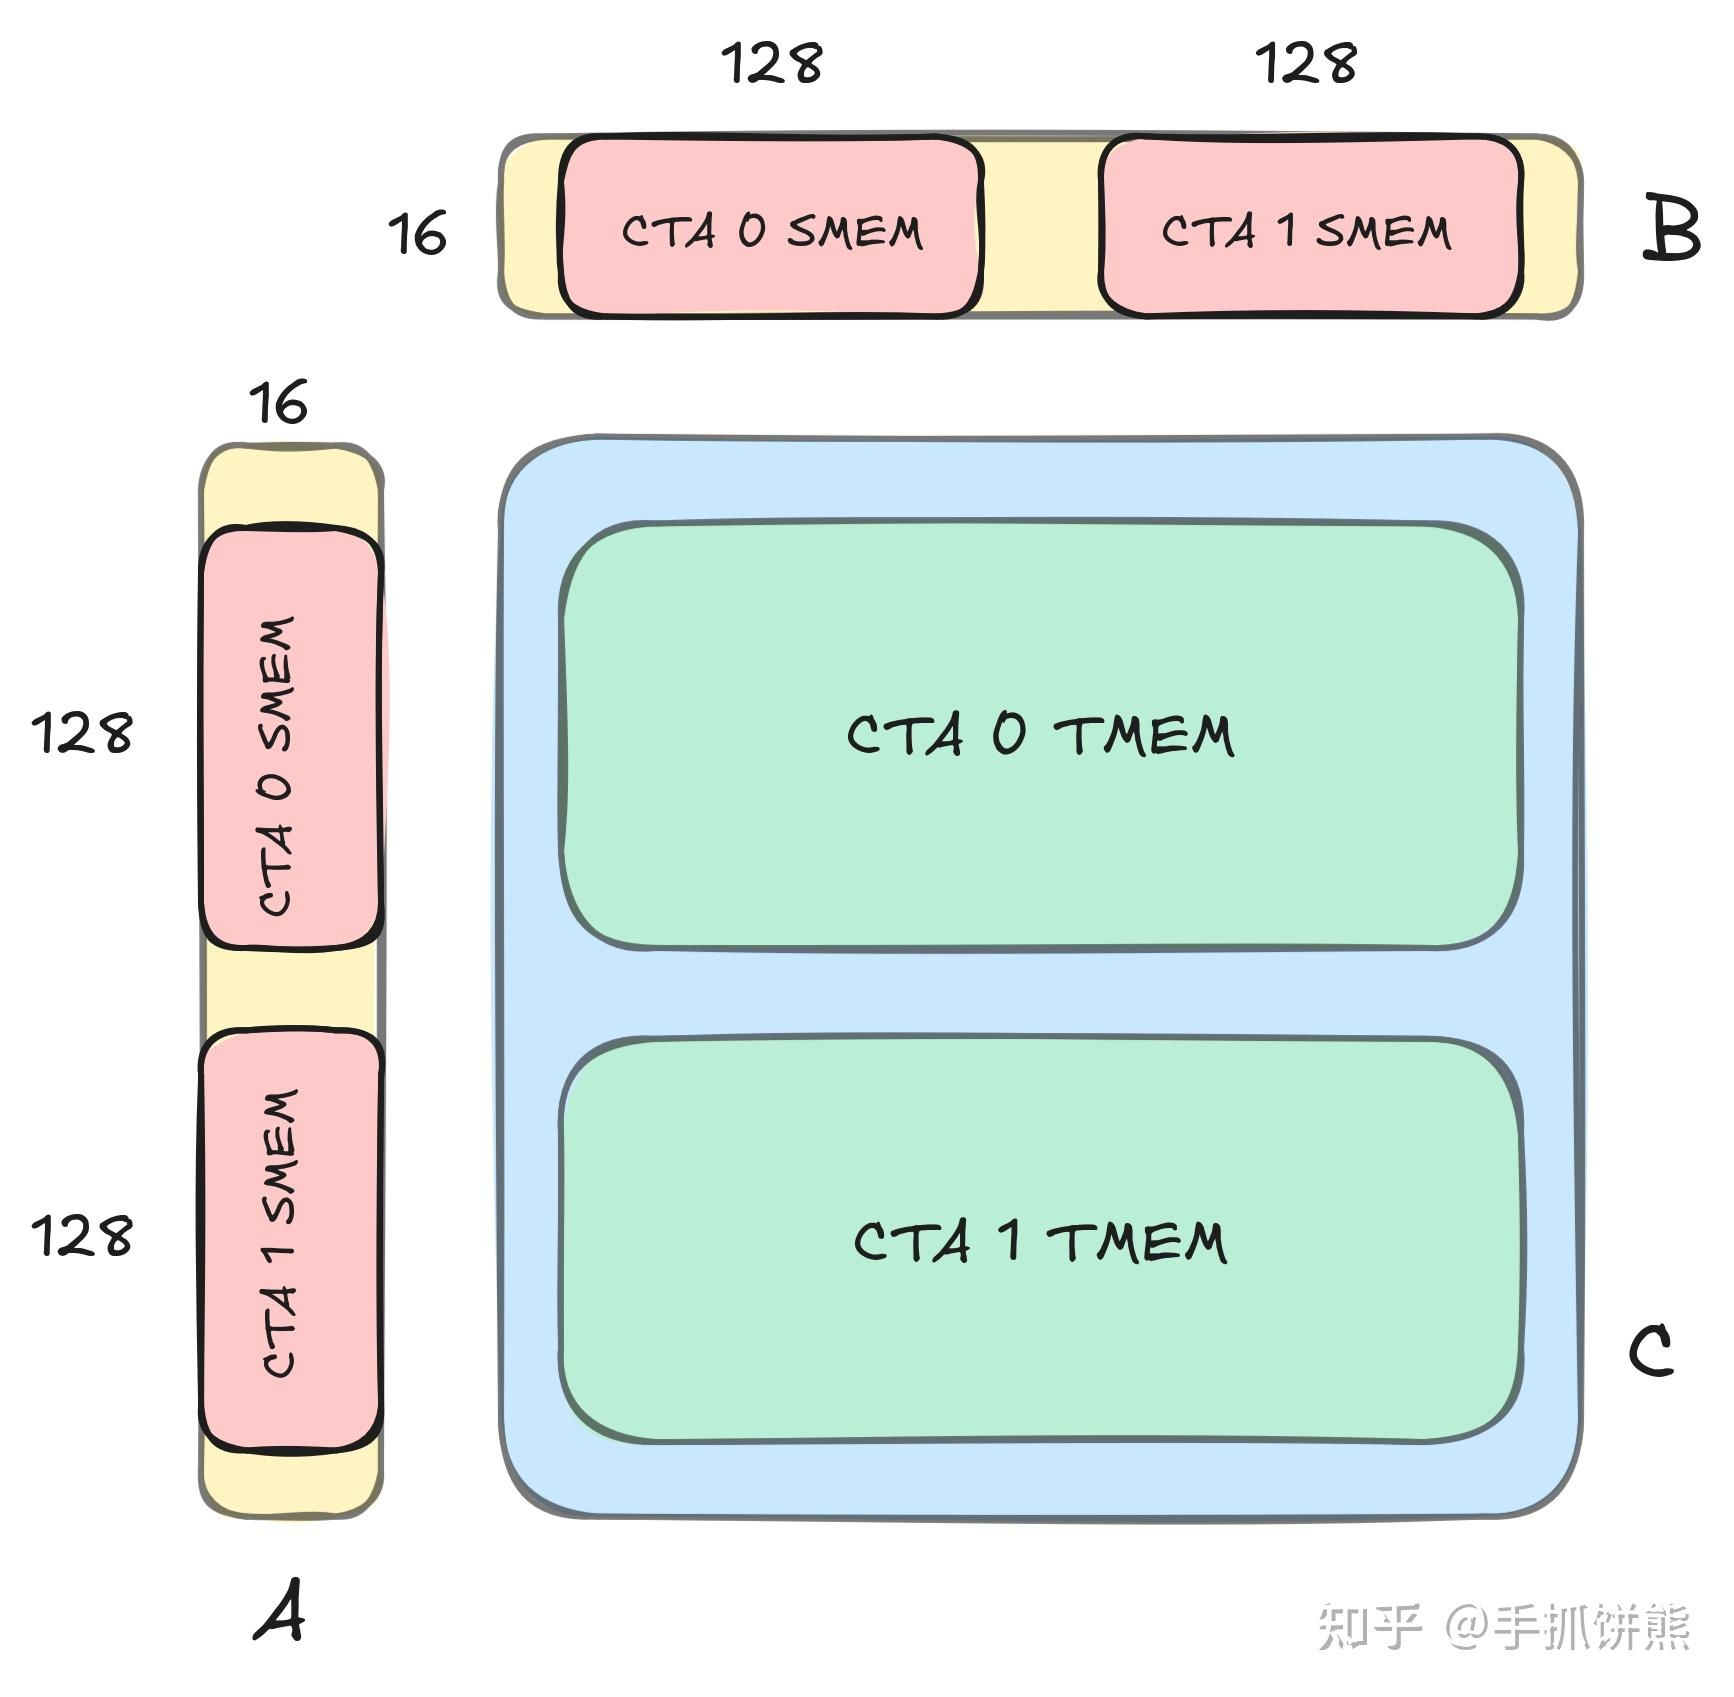
\includegraphics[width=\textwidth]{figures/zhaoshangchun-02-cluster-gemm/fig-17.jpg}
\caption{图 5. 256x256x16 pair-UMMA 的操作数切片和 TMEM 所有权。}
\end{figure}

我们在这里看到没有重叠的数据加载。因此，就算术强度而言，这确实像一个 256×256 的 MMA；与让两个 CTA 分别执行两个独立的 128×256 MMA 相比，256×256 MMA 执行相同数量的 FLOP，但传输的操作数数据量减半。

Pair-UMMA 从 PTX 发出时使用带有限定符 \texttt{cta\_\allowbreak{}group::\allowbreak{}2} 的 \texttt{tcgen05.\allowbreak{}mma} 指令。支持的 M 大小为 128 和 256，累加器总是在 M 方向上在两个 CTA 之间分割，这对选择cluster形状有一些影响。有关数据布局的更多信息，请参阅 PTX 指南。

在 CUTLASS 中，Pair-UMMA 的构造函数与单 CTA MMA 相同：

\begin{figure}[H]\centering
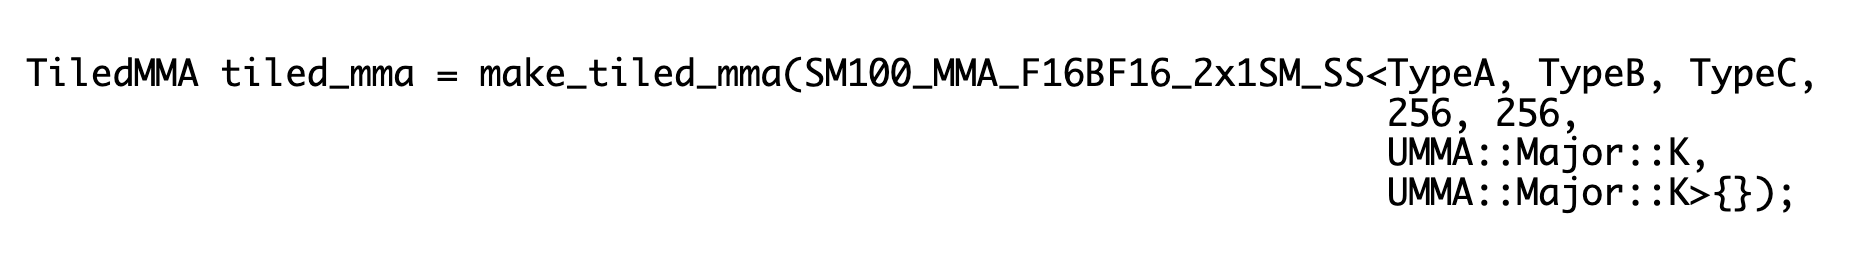
\includegraphics[width=\textwidth]{figures/zhaoshangchun-02-cluster-gemm/fig-18.png}
\end{figure}

然而，在内部，single-UMMA 和 pair-UMMA 的 \texttt{Tiled\allowbreak{}MMA} 对象之间存在许多有信息量的差异。打印出上面的 \texttt{tiled\_\allowbreak{}mma} 得到：

\begin{figure}[H]\centering
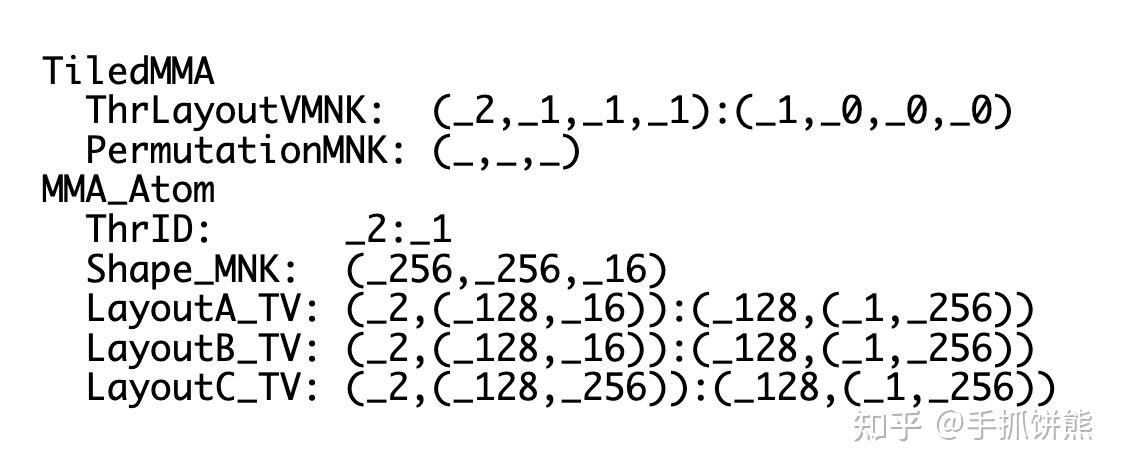
\includegraphics[width=\textwidth]{figures/zhaoshangchun-02-cluster-gemm/fig-19.jpg}
\end{figure}

正如上一篇文章所讨论的，线程索引已被重新用作 CTA 对的索引。由于这是一个 pair-UMMA，\texttt{Thr\allowbreak{}ID} 是 2，并且所有布局在第 0 个模式中相应地具有大小 2。

接下来讨论分区。每个 CTA 组与全局内存张量的一个 MMA 分片相关联，我们可以像往常一样使用 \texttt{local\_\allowbreak{}tile} 提取它：

\begin{figure}[H]\centering
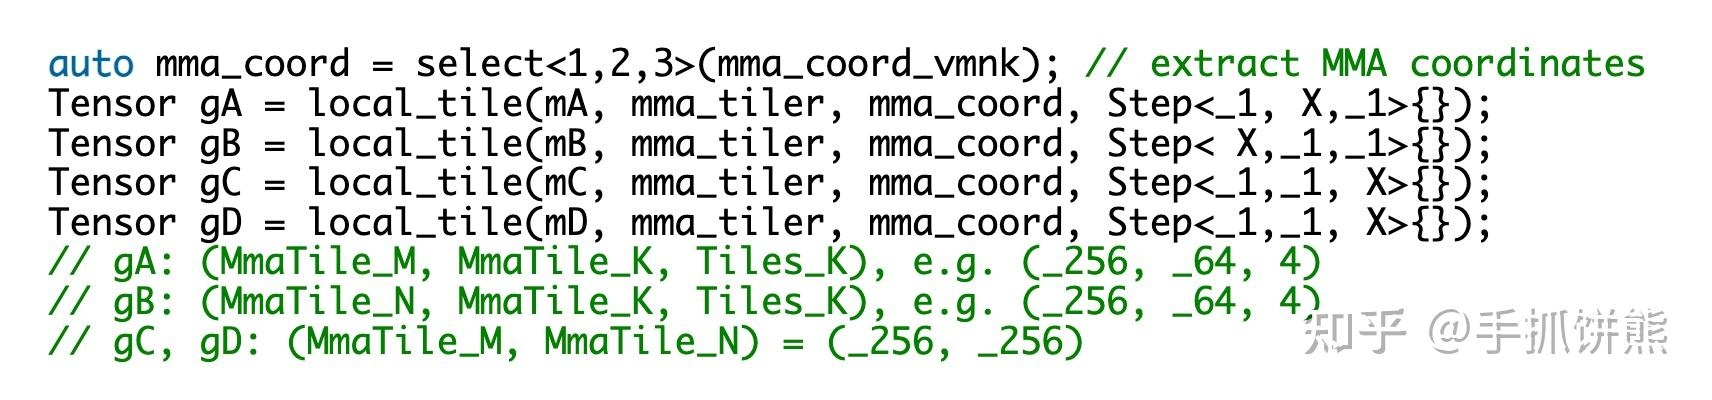
\includegraphics[width=\textwidth]{figures/zhaoshangchun-02-cluster-gemm/fig-20.jpg}
\end{figure}

然后，使用 \texttt{T\allowbreak{}h\allowbreak{}r\allowbreak{}M\allowbreak{}M\allowbreak{}A\allowbreak{}:\allowbreak{}:\allowbreak{}p\allowbreak{}a\allowbreak{}r\allowbreak{}t\allowbreak{}i\allowbreak{}t\allowbreak{}i\allowbreak{}o\allowbreak{}n\allowbreak{}\_\allowbreak{}[\allowbreak{}A\allowbreak{}|\allowbreak{}B\allowbreak{}|\allowbreak{}C\allowbreak{}]} 方法，将这些 MMA 分片在组内的 CTA 之间进行划分，以获得 CTA 本地的操作数和累加器分片。

\begin{figure}[H]\centering
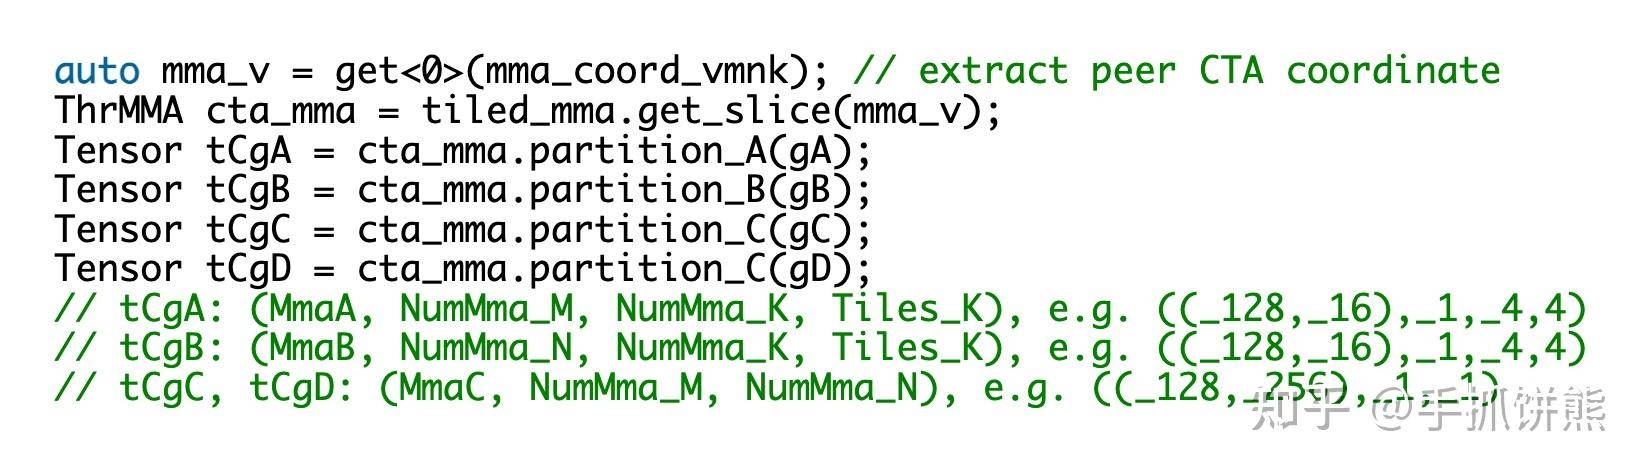
\includegraphics[width=\textwidth]{figures/zhaoshangchun-02-cluster-gemm/fig-21.jpg}
\end{figure}

一个有用的思考方式是之前的观察：CTA 坐标已经取代了线程坐标。在 Hopper 及更早版本的 GEMM 核心中加载操作数矩阵时，CTA 本地分片通过线程 ID 进行切片以提取线程本地分区。在 Blackwell 上，每个 MMA 本地分片通过对等 CTA ID 进行切片以获得 CTA 本地分区。此示例中的代码是通用编写的，也适用于 single-UMMA，在这种情况下，V 维度的大小均为 1，每个 MMA 分片包含一个 CTA 分区。

最后一点，pair-UMMA 必须从我们选为\textbf{领导 CTA} 的其中一个 CTA 中的一个线程启动；在 CUTLASS 中，我们总是选择偶数 CTA 作为领导。

\begin{figure}[H]\centering
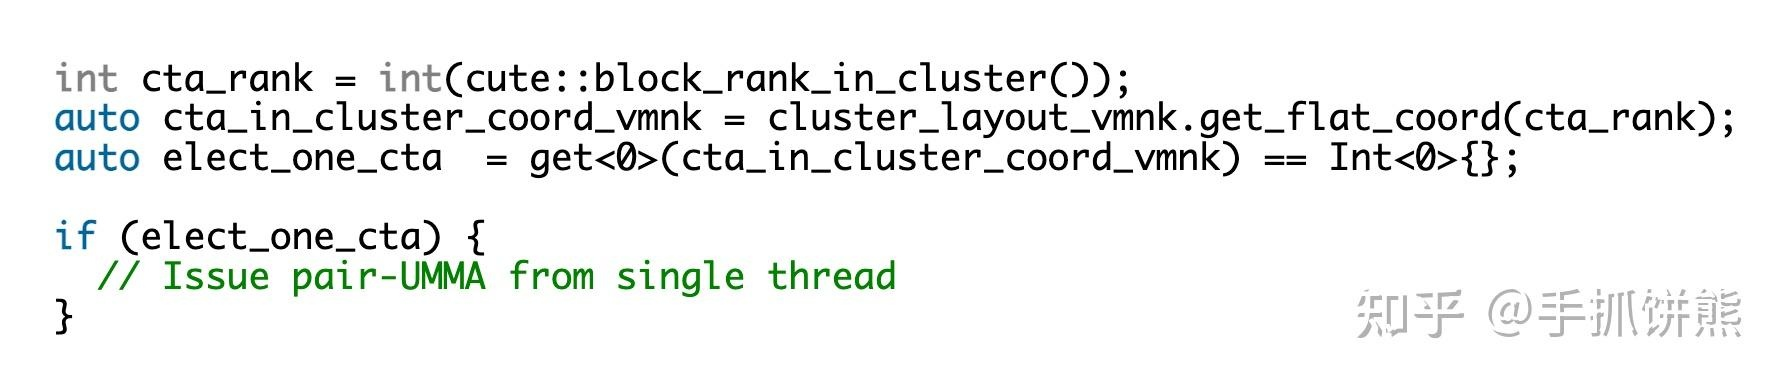
\includegraphics[width=\textwidth]{figures/zhaoshangchun-02-cluster-gemm/fig-22.jpg}
\end{figure}

\subsection{TMA 多播和 Pair-UMMA 主循环}

现在我们有了启用了 pair-UMMA 的 \texttt{tiled\_\allowbreak{}mma} 对象，让我们看看示例 4 中给出的实现。核心的主要工作流程如下：

\begin{figure}[H]\centering
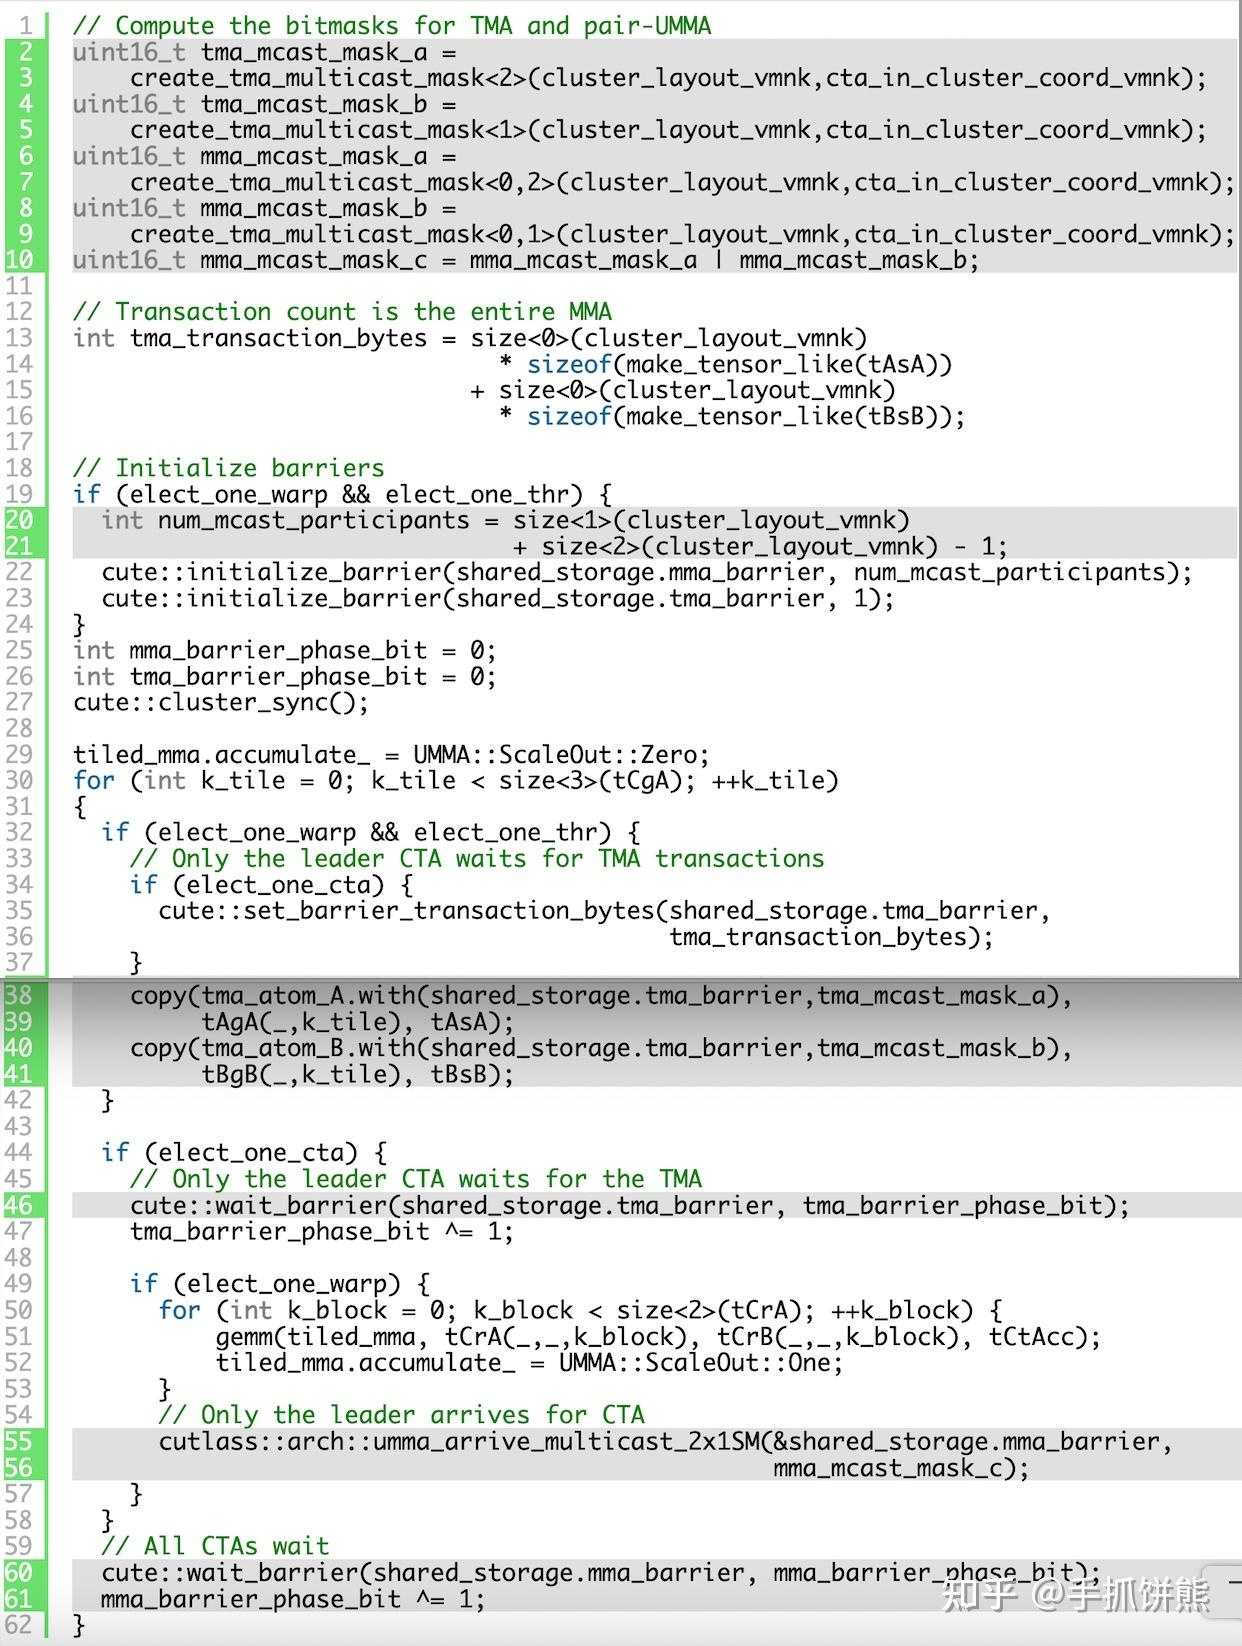
\includegraphics[height=0.85\textheight,width=\textwidth,keepaspectratio]{figures/zhaoshangchun-02-cluster-gemm/fig-23.jpg}
\end{figure}

在本节的剩余部分，我们将深入分析此示例的不同组成部分。

\subsection{构造位掩码}

首先，我们将介绍 TMA 和 MMA 位掩码。回想一下，位掩码表示 TMA 和 MMA 的数据依赖性，所以让我们从了解这与单 CTA 情况相比有何变化开始。在 2\allowbreak{}SM 情况下，每个 CTA 负责 MMA 分片的一个不重叠的一半；偶数 CTA 不需要来自奇数 CTA 的数据，反之亦然。因此，TMA 多播只需要多播到具有相同奇偶性的 CTA。另一方面，MMA 使用整个 MMA 分片，因此它需要来自两种 CTA 奇偶性的数据。这一点反映在位掩码中。

例如，在cluster形状为 \texttt{<4,\allowbreak{}4,\allowbreak{}1>}（产生形状为 \texttt{<2,\allowbreak{} 2,\allowbreak{} 4,\allowbreak{} 1>} 的四维cluster）的情况下，CTA 0 具有以下位掩码：

\begin{itemize}
\item \texttt{tma\_\allowbreak{}mcast\_\allowbreak{}mask\_\allowbreak{}a}: 0x1111
\item \texttt{tma\_\allowbreak{}mcast\_\allowbreak{}mask\_\allowbreak{}b}: 0x0005
\item \texttt{mma\_\allowbreak{}mcast\_\allowbreak{}mask\_\allowbreak{}c}: 0x333f
\end{itemize}

图 6 显示了此 pair-UMMA 示例的位掩码到 CTA 的映射。

\begin{figure}[H]\centering
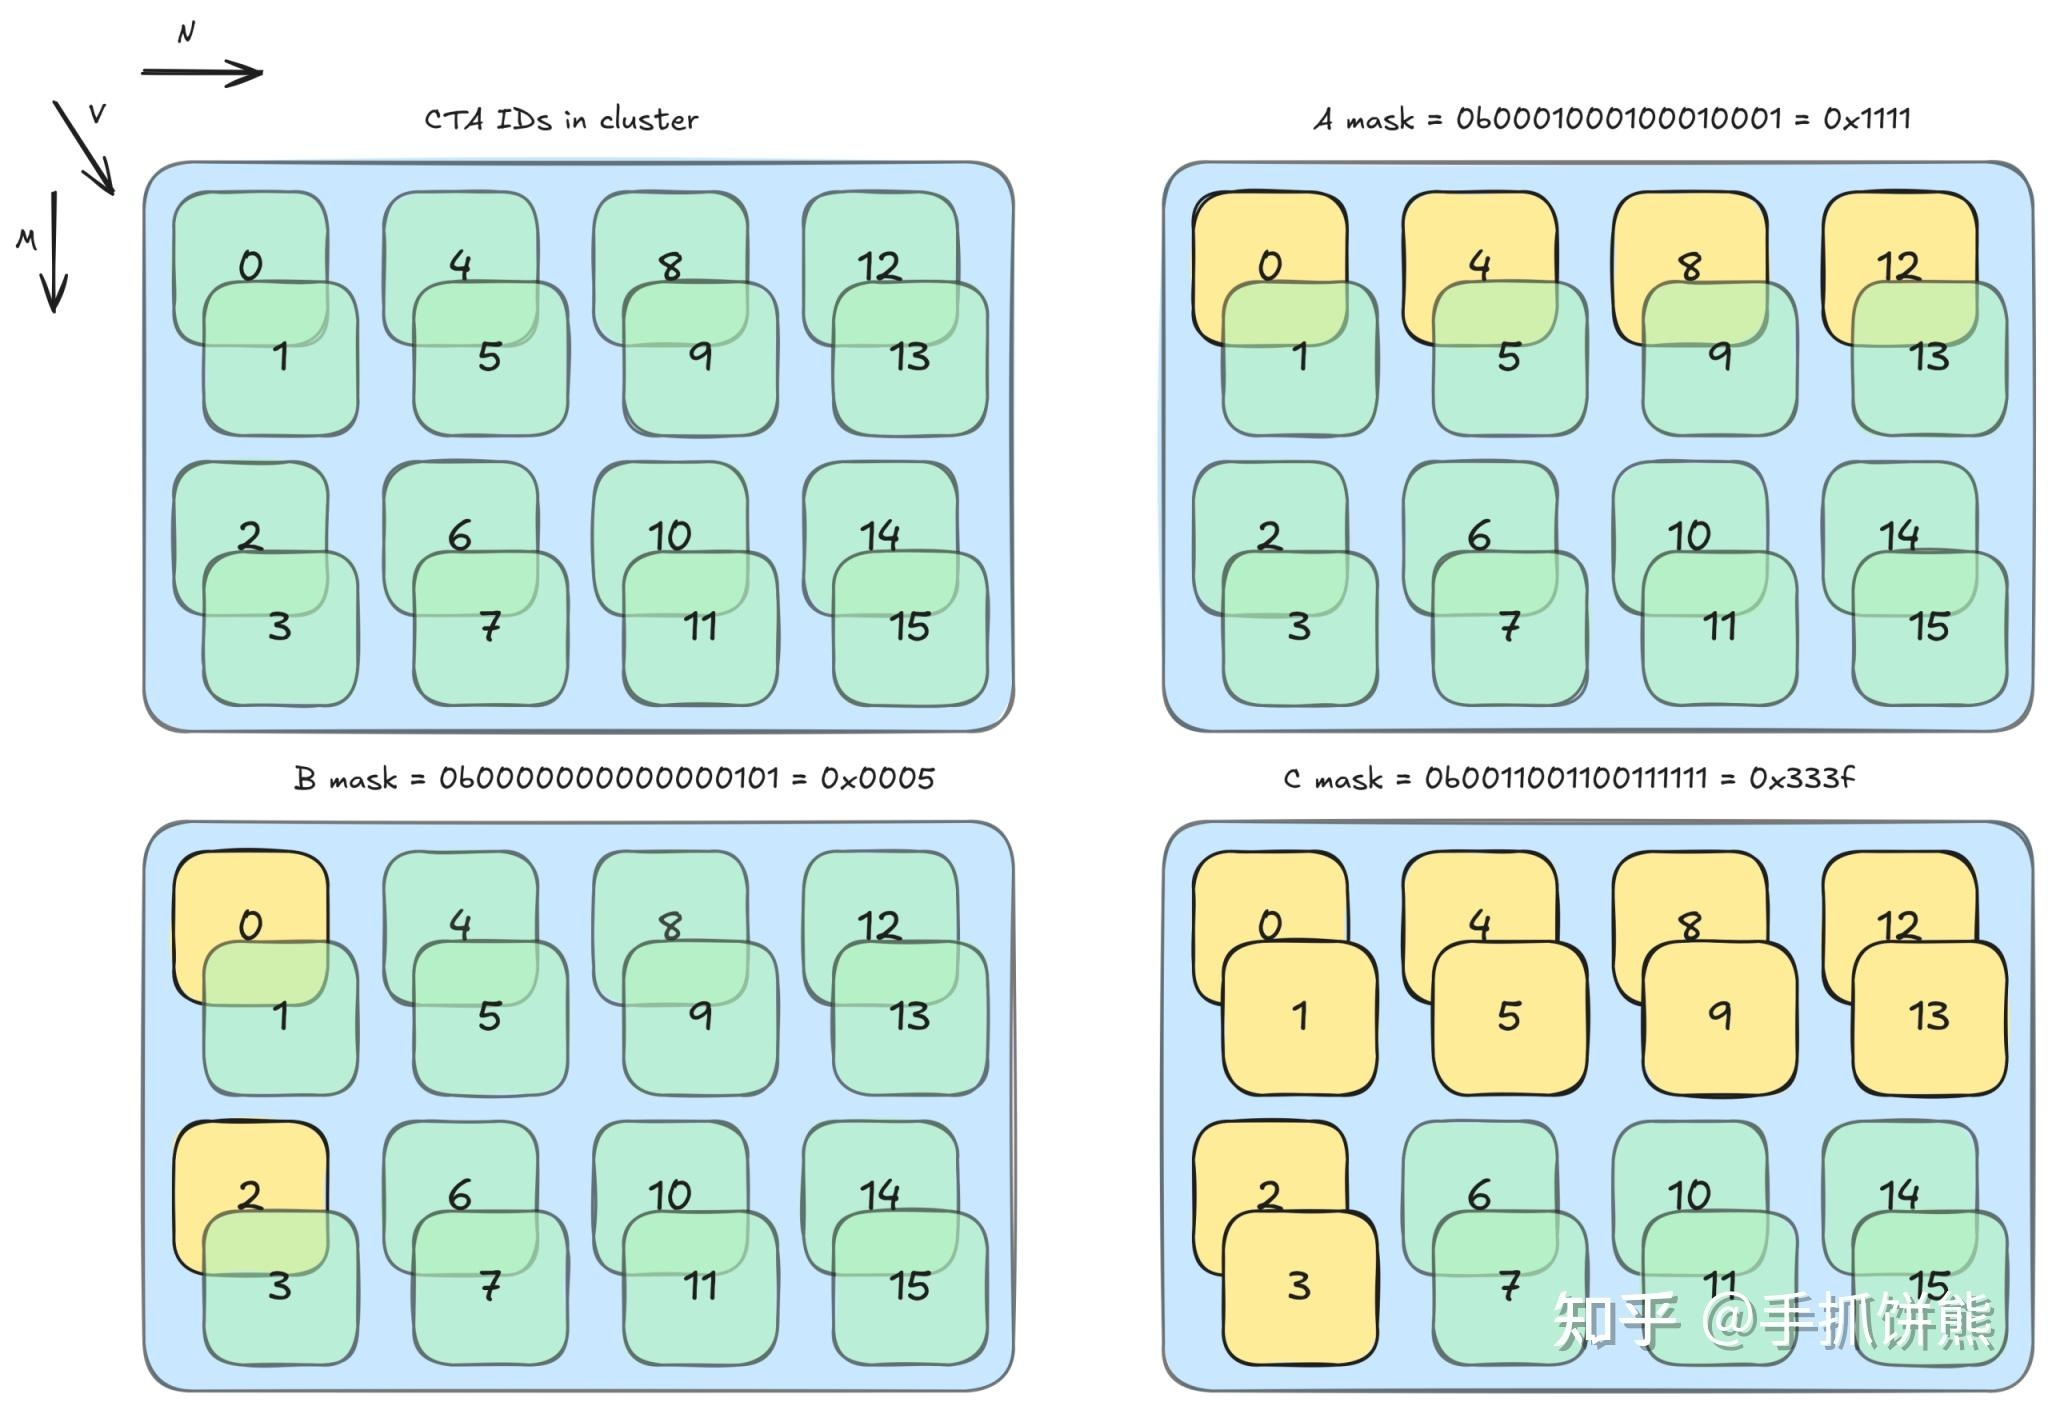
\includegraphics[width=\textwidth]{figures/zhaoshangchun-02-cluster-gemm/fig-24.jpg}
\caption{图 6. 使用 CTA 对的核心中，CTA 0 的 TMA 和 MMA 掩码。现在 CTA 在cluster中按 (V, M, N, K) 顺序组织。}
\end{figure}

对于 TMA 多播掩码，对于 CTA 0，只有行或列中的偶数 CTA 被设置为 1，因为奇数 CTA 是数据独立的。但对于 MMA，两种半数都被设置为 1，因为 MMA 使用两种半数。

要构造这些掩码，我们可以再次使用第 2-10 行中显示的 CUTLASS 实用函数。与 1 SM 情况的不同之处在于，CTA 的 MMA 位掩码不再是其 TMA 位掩码的按位 OR，而是其 TMA 位掩码与其对等体的 MMA 位掩码一起的按位 OR。一般来说，\texttt{c\allowbreak{}r\allowbreak{}e\allowbreak{}a\allowbreak{}t\allowbreak{}e\allowbreak{}\_\allowbreak{}t\allowbreak{}m\allowbreak{}a\allowbreak{}\_\allowbreak{}m\allowbreak{}u\allowbreak{}l\allowbreak{}t\allowbreak{}i\allowbreak{}c\allowbreak{}a\allowbreak{}s\allowbreak{}t\allowbreak{}\_\allowbreak{}m\allowbreak{}a\allowbreak{}s\allowbreak{}k\allowbreak{}<\allowbreak{}M\allowbreak{}o\allowbreak{}d\allowbreak{}e\allowbreak{}s\allowbreak{}.\allowbreak{}.\allowbreak{}.\allowbreak{}>\allowbreak{}(\allowbreak{}c\allowbreak{}l\allowbreak{}u\allowbreak{}s\allowbreak{}t\allowbreak{}e\allowbreak{}r\allowbreak{}\_\allowbreak{}l\allowbreak{}a\allowbreak{}y\allowbreak{}o\allowbreak{}u\allowbreak{}t\allowbreak{}\_\allowbreak{}v\allowbreak{}m\allowbreak{}n\allowbreak{}k\allowbreak{},\allowbreak{} \allowbreak{}c\allowbreak{}t\allowbreak{}a\allowbreak{}\_\allowbreak{}i\allowbreak{}n\allowbreak{}\_\allowbreak{}c\allowbreak{}l\allowbreak{}u\allowbreak{}s\allowbreak{}t\allowbreak{}e\allowbreak{}r\allowbreak{}\_\allowbreak{}c\allowbreak{}o\allowbreak{}o\allowbreak{}r\allowbreak{}d\allowbreak{}\_\allowbreak{}v\allowbreak{}m\allowbreak{}n\allowbreak{}k\allowbreak{})} 产生一个由所有 CTA 组成的位掩码，这些 CTA 与指定的 CTA 仅在cluster布局的给定模式上不同。所以 \texttt{c\allowbreak{}r\allowbreak{}e\allowbreak{}a\allowbreak{}t\allowbreak{}e\allowbreak{}\_\allowbreak{}t\allowbreak{}m\allowbreak{}a\allowbreak{}\_\allowbreak{}m\allowbreak{}u\allowbreak{}l\allowbreak{}t\allowbreak{}i\allowbreak{}c\allowbreak{}a\allowbreak{}s\allowbreak{}t\allowbreak{}\_\allowbreak{}m\allowbreak{}a\allowbreak{}s\allowbreak{}k\allowbreak{}<\allowbreak{}2\allowbreak{}>} 创建了参与此 A 分片 TMA 加载的 CTA 的掩码（这些 CTA 可能在 N 模式上与此 CTA 不同），而 \texttt{c\allowbreak{}r\allowbreak{}e\allowbreak{}a\allowbreak{}t\allowbreak{}e\allowbreak{}\_\allowbreak{}t\allowbreak{}m\allowbreak{}a\allowbreak{}\_\allowbreak{}m\allowbreak{}u\allowbreak{}l\allowbreak{}t\allowbreak{}i\allowbreak{}c\allowbreak{}a\allowbreak{}s\allowbreak{}t\allowbreak{}\_\allowbreak{}m\allowbreak{}a\allowbreak{}s\allowbreak{}k\allowbreak{}<\allowbreak{}0\allowbreak{},\allowbreak{}2\allowbreak{}>} 创建了使用此 A 分片参与 MMA 的 CTA 的掩码（这些 CTA 可能在 V 和 N 模式上与此 CTA 不同）。MMA 的最终掩码包含所有使用此 A 分片或 B 分片参与 MMA 的 CTA，即可能在 V 和 N 模式或 V 和 M 模式上不同的 CTA。

\subsection{同步 pair-UMMA}

现在让我们看看 UMMA 的同步。因为启动来自偶数 CTA，UMMA 的到达指令也必须来自偶数 CTA。因此，在创建 MMA 屏障时，mma 屏障的参与者数量是 MMA 的数量，而不是 CTA 的数量。我们在第 20-21 行看到了这一点。在 \texttt{cluster\_\allowbreak{}shape\_\allowbreak{}vmnk} 中，M 模式的大小为 2，N 模式的大小为 4。所以参与者数量（到达计数）是 5，尽管涉及 10 个 CTA。

pair-UMMA 的到达指令是使用一个特殊的 CUTLASS 函数 \texttt{u\allowbreak{}m\allowbreak{}m\allowbreak{}a\allowbreak{}\_\allowbreak{}a\allowbreak{}r\allowbreak{}r\allowbreak{}i\allowbreak{}v\allowbreak{}e\allowbreak{}\_\allowbreak{}m\allowbreak{}u\allowbreak{}l\allowbreak{}t\allowbreak{}i\allowbreak{}c\allowbreak{}a\allowbreak{}s\allowbreak{}t\allowbreak{}\_\allowbreak{}2\allowbreak{}x\allowbreak{}1\allowbreak{}S\allowbreak{}M} 发出的（见第 55-56 行）。这是因为 \texttt{tcgen05.\allowbreak{}commit} 只追踪\textbf{同一 \texttt{cta\_\allowbreak{}group}} 下先前发出的异步 tcgen05 操作：带 \texttt{cta\_\allowbreak{}group::\allowbreak{}1} 与 \texttt{cta\_\allowbreak{}group::\allowbreak{}2} 的 commit 各自追踪自己那一组。Pair-UMMA 是使用 \texttt{cta\_\allowbreak{}group::\allowbreak{}2} 限定符启动的，所以我们需要指示 \texttt{tcgen05.\allowbreak{}commit} 寻找 \texttt{cta\_\allowbreak{}group::\allowbreak{}2}。

如果对于给定的 MMA 分片，只有 5 个领导 CTA 将到达这个屏障，那为什么我们传入了一个大小为 10 的位掩码，其中也包含非领导 CTA？答案是位掩码决定了发出 CTA 到达哪些 CTA 的屏障。（请记住，由于这些 CTA 在一个cluster中，它们可以访问位于彼此共享内存中的 mbarrier。）尽管只有 5 个领导 CTA 发出 MMA 指令，但非领导 CTA 也必须等待 MMA 完成，然后才能发出下一次 TMA 拷贝并使操作数失效。我们可以在第 60-61 行看到所有 CTA 都在等待。

\subsection{为 2SM 同步 TMA 多播}

现在来看 TMA 多播同步。在第 38-41 行，TMA 以位掩码启动，该位掩码将多播限制为具有相同奇偶性的 CTA，因为每个 CTA 只负责 MMA 分片的一半。这个位掩码也意味着通常这些 TMA 只会到达具有相同奇偶性的 CTA。但是，\texttt{wait\_\allowbreak{}barrier} for TMA（第 46 行）仅从偶数 CTA 调用，并且它必须等待整个 MMA 分片。所以奇数 CTA 需要以某种方式到达偶数 CTA 的 mbarrier，尽管它们占据一个完全不相交的 TMA 位掩码。

CUTLASS 以一种有启发性的方式解决了这个问题。首先，sm100 为 TMA 拷贝指令引入了一个 \texttt{cta\_\allowbreak{}group} 限定符。将其设置为 \texttt{cta\_\allowbreak{}group::\allowbreak{}2} 允许 TMA 拷贝到达执行 CTA 或其对等 CTA 的 mbarrier。其次，此处使用的 \texttt{cute::\allowbreak{}copy} 版本通过以下方式修改 mbarrier 地址：

\begin{figure}[H]\centering
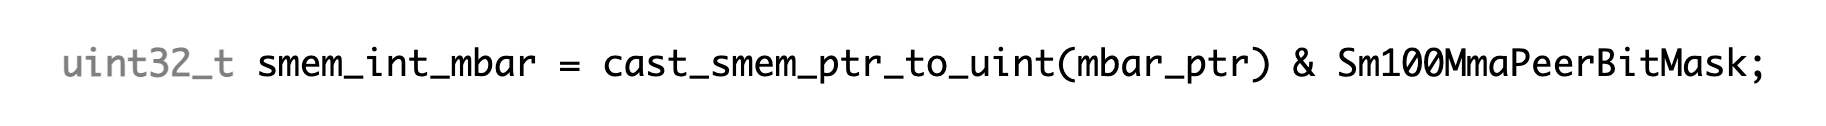
\includegraphics[width=\textwidth]{figures/zhaoshangchun-02-cluster-gemm/fig-25.png}
\end{figure}

其中 \texttt{Sm100\allowbreak{}Mma\allowbreak{}Peer\allowbreak{}Bit\allowbreak{}Mask} 是 \texttt{0x\allowbreak{}FEFFFFFF}。换句话说，一个 CTA 可以通过取其自身的 mbarrier 地址并将第 24 位设置为 0 来找到其领导 CTA 的 mbarrier 的地址。这是因为cluster中所有 CTA 的 SMEM 被视为一个单一的、统一的地址空间（对应于 PTX 的“共享状态空间”），cluster中的 CTA ID 占据地址的高位。特别地，地址的第 24 位必须对应于 CTA ID 的第 0 位，即 CTA 在其对中的索引。请注意，为此 TMA 拷贝使用 \texttt{cute::\allowbreak{}copy} 要求cluster中的所有 CTA 具有相同的共享存储布局，并要求我们采用 CUTLASS 选择偶数 CTA 作为领导的约定。

可以使用一个特殊的函数 \textbf{\texttt{m\allowbreak{}a\allowbreak{}k\allowbreak{}e\allowbreak{}\_\allowbreak{}t\allowbreak{}m\allowbreak{}a\allowbreak{}\_\allowbreak{}a\allowbreak{}t\allowbreak{}o\allowbreak{}m\allowbreak{}\_\allowbreak{}[\allowbreak{}A\allowbreak{}|\allowbreak{}B\allowbreak{}]\allowbreak{}\_\allowbreak{}s\allowbreak{}m\allowbreak{}1\allowbreak{}0\allowbreak{}0\allowbreak{}(\allowbreak{})}} 来创建一个对专用的拷贝原子，该函数与 \texttt{sm90} 接口略有不同，并且需要更多关于 UMMA 本身的细节作为参数。以下是示例 4 的原子。

\begin{figure}[H]\centering
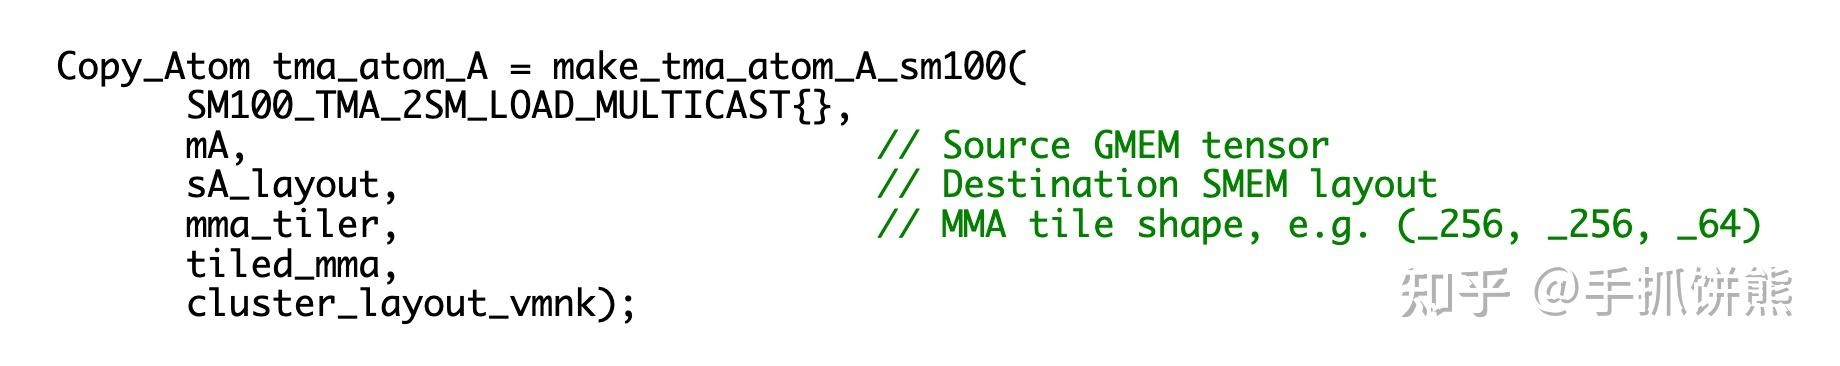
\includegraphics[width=\textwidth]{figures/zhaoshangchun-02-cluster-gemm/fig-26.jpg}
\end{figure}

请注意，与之前 1\allowbreak{}SM 情况不同，我们这里没有手动指定多播维度。相反，多播维度由 \texttt{m\allowbreak{}a\allowbreak{}k\allowbreak{}e\allowbreak{}\_\allowbreak{}t\allowbreak{}m\allowbreak{}a\allowbreak{}\_\allowbreak{}a\allowbreak{}t\allowbreak{}o\allowbreak{}m\allowbreak{}\_\allowbreak{}[\allowbreak{}A\allowbreak{}|\allowbreak{}B\allowbreak{}]\allowbreak{}\_\allowbreak{}s\allowbreak{}m\allowbreak{}1\allowbreak{}0\allowbreak{}0} 函数适当地选择。这是因为多播维度是由 MMA 原子的限制决定的，它总是在 M 方向上分割累加器。打印这个 TMA 原子，我们可以再次看到之前的线程模式被用作对等 CTA 模式。

\begin{figure}[H]\centering
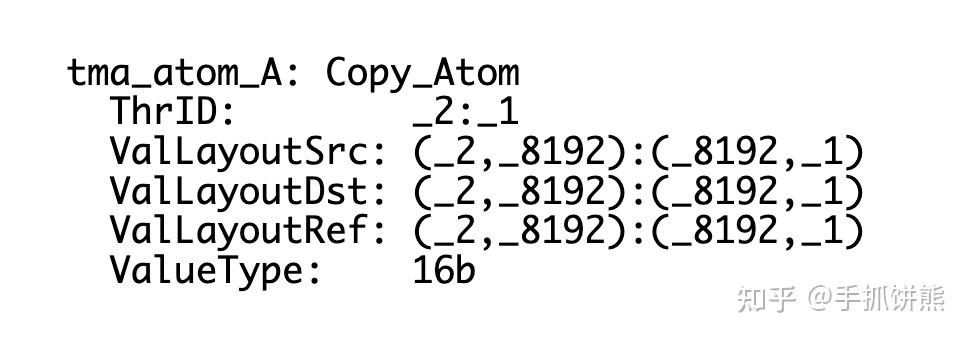
\includegraphics[width=\textwidth]{figures/zhaoshangchun-02-cluster-gemm/fig-27.jpg}
\end{figure}

这代表了两个数据无关的 128x16x4 加载（回想一下，每个 SMEM 分片我们有 4 次主循环迭代）。

\section{结论}

在这篇博客文章中，我们通过研读第 3 和第 4 个 Cu\allowbreak{}Te Blackwell 示例，考察了 NVIDIA Blackwell 架构中线程块cluster的高级用法。特别是，我们研究了 TMA 多播和 2-SM UMMA（即 pair-UMMA）。对于这两个特性，我们首先深入探讨了更精细的细节，如 PTX、索引逻辑和位掩码。然后我们研究了 CUTLASS 的实现，发现复杂的索引逻辑被 Cu\allowbreak{}Te 布局和实用函数抽象化了。

到目前为止，我们只涵盖了使用半精度数据类型的标准 GEMM。然而，Blackwell 架构增加了对低精度 GEMM 的额外支持，包括块缩放。我们将在本系列的下一篇也是最后一篇博客中讨论这个主题。

\endgroup
